\documentclass[runningheads]{llncs}

\usepackage[T1]{fontenc}
\usepackage{graphicx}
%\usepackage{color}
%\renewcommand\UrlFont{\color{blue}\rmfamily}

\usepackage{amsmath,amssymb,amsfonts}
\usepackage{algorithmic}
\usepackage[inline, shortlabels]{enumitem}
\usepackage{tabularx}
\usepackage{caption}
% \usepackage{titlesec}
\usepackage[english]{babel}
\captionsetup{font=it}
\usepackage{ragged2e}
\usepackage{hyperref}
\usepackage{pifont}
\usepackage{footmisc}
\usepackage{multirow}

% --- Tickz
\usepackage{physics}
\usepackage{amsmath}
\usepackage{tikz}
\usepackage{mathdots}
\usepackage{yhmath}
\usepackage{cancel}
\usepackage{color}
\usepackage{siunitx}
\usepackage{array}
\usepackage{multirow}
\usepackage{amssymb}
\usepackage{gensymb}
\usepackage{tabularx}
\usepackage{extarrows}
\usepackage{booktabs}
\usetikzlibrary{fadings}
\usetikzlibrary{patterns}
\usetikzlibrary{shadows.blur}
\usetikzlibrary{shapes}

% ---------

\usepackage{pdfpages}
\usepackage{booktabs}
\usepackage{csquotes}
\usepackage{lipsum}  
\usepackage{arydshln}
\usepackage{smartdiagram}
\usepackage[inkscapeformat=png]{svg}
\usepackage{textcomp}
\usepackage{tabularray}\UseTblrLibrary{varwidth}
\usepackage{xcolor}
\def\BibTeX{{\rm B\kern-.05em{\sc i\kern-.025em b}\kern-.08em
    T\kern-.1667em\lower.7ex\hbox{E}\kern-.125emX}}
\usepackage{cite}
\usepackage{amsmath}
\newcommand{\probP}{\text{I\kern-0.15em P}}
\usepackage{etoolbox}
\patchcmd{\thebibliography}{\section*{\refname}}{}{}{}

\setlength{\extrarowheight}{2.5pt}

\renewcommand{\arraystretch}{1.7}

\setlength{\extrarowheight}{2.5pt}
\renewcommand{\arraystretch}{0.2}
\renewcommand{\arraystretch}{1.7}

% --------------
% \titleclass{\subsubsubsection}{straight}[\subsection]

% \newcounter{subsubsubsection}[subsubsection]
% \renewcommand\thesubsubsubsection{\thesubsubsection.\arabic{subsubsubsection}}
% \renewcommand\theparagraph{\thesubsubsubsection.\arabic{paragraph}} % optional; useful if paragraphs are to be numbered

% \titleformat{\subsubsubsection}
%   {\normalfont\normalsize\bfseries}{\thesubsubsubsection}{1em}{}
% \titlespacing*{\subsubsubsection}
% {0pt}{3.25ex plus 1ex minus .2ex}{1.5ex plus .2ex}

% \makeatletter
% \renewcommand\paragraph{\@startsection{paragraph}{5}{\z@}%
%   {3.25ex \@plus1ex \@minus.2ex}%
%   {-1em}%
%   {\normalfont\normalsize\bfseries}}
% \renewcommand\subparagraph{\@startsection{subparagraph}{6}{\parindent}%
%   {3.25ex \@plus1ex \@minus .2ex}%
%   {-1em}%
%   {\normalfont\normalsize\bfseries}}
% \def\toclevel@subsubsubsection{4}
% \def\toclevel@paragraph{5}
% \def\toclevel@paragraph{6}
% \def\l@subsubsubsection{\@dottedtocline{4}{7em}{4em}}
% \def\l@paragraph{\@dottedtocline{5}{10em}{5em}}
% \def\l@subparagraph{\@dottedtocline{6}{14em}{6em}}
% \makeatother

% \setcounter{secnumdepth}{4}
% \setcounter{tocdepth}{4}
% --------------

\newcommand{\before}[1]{\textcolor{red}{#1}}
\newcommand{\after}[1]{\textcolor{green}{#1}}

\newcommand{\old}[1]{\textcolor{orange}{#1}}
\newcommand{\rem}[1]{\textcolor{red}{#1}}
\newcommand{\todo}[1]{\textcolor{orange}{\newline \textit{\textbf{TODO:} #1}} \newline \newline }


% --------------------------------
%             DOCUMENT
% --------------------------------

\begin{document}
%
\title{An Approach for Multi-Agent System Design with Reinforcement Learning}
%
%\titlerunning{Abbreviated paper title}
% If the paper title is too long for the running head, you can set
% an abbreviated paper title here
%
\author{Julien Soulé\inst{1}\orcidID{0000-1111-2222-3333} \and
    Jean-Paul Jamont\inst{1}\orcidID{1111-2222-3333-4444} \and
    Michel Occelo\inst{1}\orcidID{2222--3333-4444-5555} \and
    Louis-Marie Traonouez\inst{2}\orcidID{2222--3333-4444-5555} \and
    Paul Théron\inst{3}\orcidID{2222--3333-4444-5555}}
%
\authorrunning{J. Soulé et al.}
% First names are abbreviated in the running head.
% If there are more than two authors, 'et al.' is used.
%
\institute{Univ. Grenoble Alpes, Grenoble INP, LCIS, 26000, Valence, France
    \email{\{julien.soule, jean-paul.jamont, michel.occello\}@lcis.grenoble-inp.fr}
    \and
    Thales Land and Air Systems, BU IAS, Rennes, France
    \email{louis-marie.traonouez@thalesgroup.com}
    \and
    AICA IWG, La Guillermie, France \\
    \email{paul.theron@orange.fr}
}
%
\maketitle              % typeset the header of the contribution
%
\begin{abstract}

    % context
    Multi-Agent Reinforcement Learning has been successfully applied in various contexts to generate policies allowing agents to collaboratively achieve a goal in a non-fully observable environment. These policies are approximated functions that map observation to action allowing agents to maximize the cumulative reward over an episode.
    % problem
    Yet, from a designer point of view, those trained policies raise explainability and safety issues because they do not give human-understandable or exploitable specifications of their organizational aspects such as individual, social or collective levels.
    % This particularly concerns black box models in deep-learning or random forest.
    % hypothesis / contribution
    This paper aims to define the organizational explainability problem formally. Then, we expose our approach to extract the organization specifications out of trained agents policies.
    % results
    We applied our approach in three manageable cooperative Atari games likely to have emergent organization among agents. Resulting organization specifications are indeed consistent with human expectations.
    
    \keywords{Multi-Agent Systems \and Reinforcement Learning \and Organization \and Design}
\end{abstract}

\section{Introduction}

% Context
In Multi-Agent Systems (MASs), organization is a fundamental concept that impact how agents are coordinating their activities to collaboratively achieve a common goal~\cite{Hubner2002}. In essence, we assume the entity of the organization (we simply call \textbf{organization}) always exists through the running agents interactions even though it may be implicit.
An \textbf{organizational model} specifies (at least partially) the organization whether it is used as medium to describe an explicit known organization in a top-down way, or describing an implicit organization in a bottom-up way. Examples of organizational models are the Agent/Group/Role (AGR) model~\cite{Ferber2004} or more complex ones such as $\mathcal{M}OISE^{+}$~\cite{Hubner2002}. Organizational models can take into account aspects such as structural coordination, dynamic interactions, and the achievement of common objectives~\cite{Ferber2004, Abbas2015}. We call the \textbf{specifications} of an organization, the set of components used in an instance of an organizational model to specify the organization.

We assume an organization in a MAS can be understood regarding the Agent Centered Point of View (ACPV) vs. Organization Centered Point of View (OCPV) and agent's organization awareness vs. unawareness~\cite{Picard2009}.
Typical examples are emergent MAS (ACPV and organization unawareness), coalition based MAS (ACPV and organization awareness), organization based MAS (OCPV and organization awareness), and Agent oriented engineering (OCPV and organization unawareness)~\cite{Picard2009}.
We assume an \textbf{architecture} (also called organizational paradigm) is an abstract organization gathering a range of organizations sharing common characteristics~\cite{Horling2004}. Finally, MAS designing/development methods, have been proposed jointly with organizational models to help designers finding suited specifications of an organization so a MAS can reach a goal efficiently in a environment such as GAIA~\cite{Wooldridge2000}, ADELFE~\cite{Bernon2003} or DIAMOND~\cite{Jamont2005}.

In most \textbf{self/re-organization} mechanisms agents' policies are defined and fixed by the designer from ACPV/OCPV so that an optional emerging/chosen organization allows reaching a global goal~\cite{Picard2009}. We can envision Multi-Agent Reinforcement Learning (MARL) as a particular ACPV mechanism that aims to replace the designer by simultaneously making emerge agents' policies (micro-level) and consequently the emerging organization (macro-level) relying on quantitative feedbacks. In literature, that mechanism is mostly considered to satisfy the need that agents reach efficiently a specific goal with few other considerations. Typical examples include agents' policies modeled as neural networks that are updated using various algorithms such as Deep Q-Network or REINFORCE. In such examples, an emerging implicit organization among agents can converge.

In some environments, such as computers network with highly complex and non-visual interactions, the lack of intuitive comprehension of the environment can make MAS methods difficult to apply to develop a MAS whose organization optimally reach a goal. In such cases, the use of MARL could allow to have sufficiently and non over-fitted trained agents optionally respecting additional arbitrary designer's constraints (coming from a architecture for instance). We think an observer/designer could understand, interpret, and produce the specifications of valuable organizations by translating them into organizational models. For instance determining the individual, social, collective levels described in $\mathcal{M}OISE^{+}$~\cite{Hubner2002}. At least it may give relevant insights for guiding the design process.

% Problem
The idea of benefitting of the particularly adaptive and general MARL mechanism to get an approximated suited MAS organization and producing associated specifications, requires to link the MARL training of a set of policies in a bidirectional way with a MAS organizational model. For instance, a hierarchy described in a MAS model would constrain the possible policies to get ultimately trained in MARL. Reversely, a set of trained policies could be described in an organizational model, thus indicating resemblance with known MAS organization architectures.

% Contribution/Hypothesis
This paper first aims to formalize the aforementioned idea through a formal model. That formal model aims to unify the concepts and links between agents' policies, their training with MARL, architecture with the $\mathcal{M}OISE^{+}$ organizational model. Relying on that formal model, we expose our approach to generate an efficient organization and associated OCPV specifications based on the environment, the initial agents' policies models, the design constraints, and the global goal.

% Results
We applied our approach to three simple Atari games involving several agents that must converge to a specific organization to achieve a goal efficiently. Obtained organization specifications are exploitable and coherent with human expectations.

The remainder of the article is built as following.
In section II, after briefly introducing the premise of the underlying idea linking organizational models and MARL. The related works we identified shows the originality of our positioning in literature.
In section III, we introduce a formal model to properly formalize our idea by linking MAS and MARL related concepts.
In section IV, we present our approach to help designers in designing a suited organization regarding environment, goal, agents' policy model and design constraints.
In section V, we discuss results obtained after applying our approach in three simple cooperative Atari games.
In section VI, we conclude on the viability and relevance of our model and approach and we highlight limitations to overcome and future works as well.

\section{Overview of the underlying idea and related works}

Whether adopting OCPV or ACPV, when designing a MAS, the human designer has to define the logic in agents themselves intending the MAS to reach some specific goals via some kind of emergent or expected organization pattern. It often takes place as an iterative process where designer are proceeding by trial and error. Despite the designer skills, that process may be hard and costly to converge towards a sufficiently estimated successful MAS. That process gets more difficult when the target deployment environment is not easily readable or handleable due to the complexity and internal safety policies such as for company infrastructure networks. Additionally, unexpected emergent phenomena may appear without giving guarantees for safety. We refer to that observation as the \textquote{human-based design difficulty}.

Instead of adopting a risky direct empiric approach, a common approach is to rely on a intermediary step by simulating the target deployment system, analogous to \textquote{digital twins}. Indeed, simulation can provide a monitoring framework that leaves room for a safe design process, while having an assessment of the resulting MAS designs. If the simulation is close enough to the target system in terms of fidelity, then we can expect the designed MAS to be transferred to the target system for indeed reaching the goals.
In that respect, creating a MAS that aims to reach a goal in any given environment, firstly focuses on finding a suited MAS design only in the associated simulation. We also, hypothesized the simulation to allow RL techniques and to give, at least, raw description of the current environment and agents states.

The premise of our idea is to benefit of a MARL process that would automatically converge to an optimal solution as for establishing the rules in agents (called \textbf{policies}) that drives the MAS to the goal. Yet, unlike human-based design where the agent's logic is explicitly specified, trained policies with MARL are approximated by black box functions such as Neural Networks. Therefore, we also need to address the explainability issue not only for individual agents' policies but for the joint-policy in its entirety through a collective point-of-view. We think, this problem can be partially addressed by considering that a joint-policy can be (at least partially) described in terms of the organizational specifications. We refer to that approach under the term of \textquote{Organization Oriented MARL} (OOMARL).

% TODO: à mettre plus tard comme un choix justifié. Ici il faut surtout parler de tous les travaux liant MARL et organisation/stratégies collectives...
Among, the existing organizational models \textquote{Agent/Group/Role}~\cite{Ferber2004} and $\mathcal{M}OISE^+$~\cite{Hubner2002} provide a relevant high-level description of the structures and interactions within the MAS. However, we favor $\mathcal{M}OISE^+$ because it provides an advanced formal description for an organization without incompatibilities with MARL, especially for formal description of agents' policies. It takes into account explicitly the social aspects between agents where \textquote{AGR} focuses on the integration of standards oriented towards design. Additionally, it provides a sufficiently detailed vision of organization to be understood at different point of views.

We think OOMARL is positioned at the crossroads of MAS and MARL and can be envisioned as a mixed ACPV/OCPV organization mechanism with no organization awareness. It falls into the broad topic of explainability in AI at an organizational level within MARL. In order to appreciate OOMARL positioning in literature, we chose the following boolean keywords formula we think better describe OOMARL:
\begin{gather*}
    ("multi" \land "agent") \land ("reinforcement \ learning")\\ \land ("explainability" \lor ("organization" \lor "collective"))
\end{gather*}

We identified few article dealing with a multi-agent vision of explainability. Most notable ones are:

% Collective explainable AI: Explaining cooperative strategies and agent contribution in multiagent reinforcement learning with shapley values
\cite{Heuillet2022} proposes a novel approach to explain cooperative strategies in multiagent reinforcement learning (RL) using Shapley values, a game theory concept used in eXplainable AI (XAI). The study aims to make deep RL more comprehensible and address the need for methods that provide better understanding and interpretability. The experimental results on Multiagent Particle and Sequential Social Dilemmas demonstrate the effectiveness of Shapley values in explaining the rationale behind decisions taken by agents. However, the article also highlights that Shapley values can only provide general explanations about a model and cannot explain specific actions taken by agents. The authors suggest that future work should focus on addressing these limitations. The study's implications extend to areas such as non-discriminatory decision making, ethical and responsible AI-derived decisions, and policy making under fairness constraints.

% Magent: A many-agent reinforcement learning platform for artificial collective intelligence
\cite{Zheng2018} presents MAgent, a platform for many-agent reinforcement learning (MARL) that aims to facilitate research on artificial collective intelligence. MAgent provides a flexible and efficient environment for training and evaluating MARL algorithms, enabling the study of complex multi-agent behaviors. The platform supports various scenarios, including cooperative, competitive, and mixed environments, and offers a high degree of scalability to accommodate a large number of agents. MAgent also includes a comprehensive set of baselines and evaluation metrics to benchmark the performance of MARL algorithms. The research contributes to the advancement of collective intelligence and the development of robust multi-agent systems.

% Self-Organized Group for Cooperative Multi-agent Reinforcement Learning
\cite{Shao2022} introduces a method called Self-Organized Group (SOG) for cooperative multi-agent reinforcement learning. In this approach, a certain number of agents are randomly elected to be conductors, and the corresponding groups are constructed with conductor-follower consensus, allowing the groups to be re-organized at regular intervals. The organized group under the unified command of a conductor is found to embed the multi-agent system with stronger zero-shot generalization ability compared to traditional methods. The SOG method provides strong adaptability to scenarios with varying numbers of agents and varying agent sight. The paper presents this approach as a mechanism to enhance cooperative multi-agent tasks with dynamic characteristics, aiming to improve the adaptability and generalization of multi-agent reinforcement learning systems

% A multi-agent reinforcement learning model of common-pool resource appropriation
\cite{Perolat2017} introduces a model that focuses on common-pool resource appropriation, a multi-agent social dilemma that includes issues such as sustainable use of fresh water, common fisheries, grazing pastures, and irrigation systems. The model emphasizes the importance of trial-and-error learning in addressing the challenges of common-pool resource sustainability and inequality. It explores the emergent behavior of groups of independently learning agents in a partially observed Markov game, shedding light on the relationship between exclusion, cooperation, and sustainability in the context of resource appropriation. The research highlights the potential of deep reinforcement learning in understanding and addressing complex societal and environmental challenges related to common-pool resource management. The paper provides valuable insights into the application of multi-agent reinforcement learning in the context of real-world social dilemmas and resource management

% MARLeME: A Multi-Agent Reinforcement Learning Model Extraction Library
\cite{Kazhdan2020} introduces MARLeME, a library designed to enhance the explainability of Multi-Agent Reinforcement Learning (MARL) systems by approximating them with symbolic models. The library aims to improve the interpretability of MARL systems, which is crucial for understanding the behavior of multiple agents interacting in a shared environment. By providing a means to extract symbolic models from MARL systems, MARLeME contributes to the advancement of explainable AI in the context of multi-agent systems.

% ROMA: Multi-Agent Reinforcement Learning with Emergent Roles
\cite{Wang2020} introduces a role-oriented MARL (Multi-Agent Reinforcement Learning) approach where roles are emergent, and agents with similar roles tend to share their learning and specialize in certain sub-tasks. The framework aims to combine the flexibility and adaptability of MARL with the concept of roles, allowing agents with similar roles to exhibit similar behaviors. The approach is designed to learn specialized, dynamic, and identifiable roles without relying on predefined role structures and behaviors. The research provides a novel perspective on the application of role-oriented MARL in complex multi-agent systems, offering potential advancements in the field of reinforcement learning.

% Promoting Coordination through Policy Regularization in Multi-Agent Deep Reinforcement Learning
\cite{Roy2020} addresses the challenge of inducing coordination between agents in multi-agent reinforcement learning. The research investigates the use of policy regularization to promote inter-agent coordination and discusses two approaches based on inter-agent modeling and synchronized sub-policy selection. The proposed methods are designed to improve cooperative behaviors without relying on explicit communication channels, allowing agents to exhibit coordinated behaviors during testing when acting in a decentralized fashion. The paper presents two policy regularization methods, TeamReg and CoachReg, and evaluates their performance on challenging cooperative multi-agent problems, showing improved results. The research contributes to the advancement of coordination-driven multi-agent approaches in reinforcement learning and provides valuable insights into promoting inter-agent coordination through policy regularization.

% Social Influence as Intrinsic Motivation for Multi-Agent Deep Reinforcement Learning
\cite{Jaques2019} proposes a mechanism for achieving coordination and communication in Multi-Agent Reinforcement Learning (MARL) by rewarding agents for having causal influence over other agents' actions. This causal influence is assessed using counterfactual reasoning, where agents simulate alternate actions to compute their effect on the behavior of other agents. The paper demonstrates that this approach leads to enhanced coordination and communication, as well as more meaningful learned communication protocols. The proposed method is shown to significantly increase the learning curves of the deep reinforcement learning agents, leading to more diversified team behavior and more successful performance of the population as a whole. The paper also highlights that the influence rewards for all agents can be computed in a decentralized way, opening up new opportunities for research in this area.

% Efficient multi-agent reinforcement learning through automated supervision
\cite{Chongjie2008} proposes a unified mechanism for achieving coordination and communication in Multi-Agent Reinforcement Learning (MARL). The approach involves training multiple agents to independently maximize their own individual reward without sharing weights. The paper introduces a method for automated supervision, which enables the agents to learn to coordinate and communicate effectively. This automated supervision mechanism leads to enhanced coordination, communication, and more meaningful learned communication protocols, ultimately improving the learning curves of the deep reinforcement learning agents and the overall performance of the agent population

% A unified framework for reinforcement learning, co-learning and meta-learning how to coordinate in collaborative multi-agent systems
\cite{Tosic2010} presents a comprehensive framework for addressing coordination in collaborative multi-agent systems. The framework integrates reinforcement learning, co-learning, and meta-learning to enable agents to learn how to coordinate effectively. By leveraging this unified approach, the paper aims to enhance the coordination and communication capabilities of multi-agent systems, ultimately improving their overall performance. 

Beside, these works explainability in RL is also widely considered in individual agents but are thought to be useful to understand the global organization. Among those works, most notable ones are:

Rule extraction from trained neural networks: involves obtaining human-interpretable rules that approximate the policy of the neural network. Various algorithms have been developed for this task, including decompositional, pedagogical, and eclectics approaches. These algorithms aim to provide comprehensible descriptions of the network's hypothesis that closely approximate its policy. For example, NN2Rules is a decompositional approach that extracts a set of decision rules from the parameters of the trained neural network model, making the decision rules more interpretable. Rule extraction algorithms enable neural networks to justify their classification responses using explainable classification rules, enhancing the transparency and interpretability of the models~\cite{Hailesilassie2016}~\cite{Sato2001}~\cite{Lal2022}.

Specification-Guided Reinforcement Learning (SGRL): addresses the problem of generating an optimal policy in reinforcement learning (RL) with respect to a given task in an unknown environment. Traditionally, the task is encoded in the form of a reward function, which can be cumbersome for long-horizon goals. An alternative approach is to use logical specifications, such as Linear Temporal Logic (LTL) and SpectRL, to define the task, opening the direction of RL from logical specifications. SGRL aims to synthesize control policies for robotic systems and other autonomous agents by leveraging formal logical constructs to express the task or objective. This approach has led to the development of highly performant algorithms that enable RL from logical specifications, enhancing the transparency and trustworthiness of RL systems~\cite{Bansal2022}~\cite{Jothimurugan2023}.

Learning from Logical Specifications: covers the broader area of learning from logical specifications, including the development of reinforcement learning algorithms that leverage the compositional structure of the specification to learn control policies for complex tasks~\cite{Jothimurugan2021}.


\section{A formal model for linking MAS and MARL concepts}

The proposed model aims to integrate MAS organization designing process by translating the $\mathcal{M}OISE^{+}$ organizational model within the formalism used for MARL. Then, we formally describe how agents' policies and training process can be linked to the $\mathcal{M}OISE^{+}$ organizational model.

\subsection{MARL model}

The chosen MARL model is based on the Decentralized Partially Observable Markov Decision Process (Dec-POMDP)~~\cite{Oliehoek2016} because it considers multiple agents in a similar MAS fashion. It relies on stochastic processes to model uncertainty of the environment for the changes induced by actions, in received observations, in communication\dots Additionally, unlike Partially Observable Stochastic Games (POSG), the reward function can be common to agents which fosters training for collaborative oriented actions~\cite{Beynier2013}.
A Dec-POMDP is a 7-tuple $(S,\{A_i\},T,R,\{\Omega_i\},O,\gamma)$, where:
\begin{itemize}
    \item $S = \{s_1, ..s_{|S|}\}$: The set of the possible states.
    \item $A_{i} = \{a_{1}^{i},..,a_{|A_{i}|}^{i}\}$: The set of the possible actions for agent $i$.
    \item $T$ so that $T(s,a,s') = \probP{(s'|s,a)}$ : The set of conditional transition probabilities between states
    \item $R: S \times A \times S \rightarrow \mathbb{R}$: The reward function
    \item $\Omega_{i} = \{o_{1}^{i},..,o_{|\Omega_{i}|}^{i}\}$: The set of observations for agent $ag_i$
    \item $O$ so that $O(s',a,o) = \probP{(o|s',a)}$ : The set of conditional observation probabilities.
    \item $\gamma \in [0,1]$, the discount factor
\end{itemize}

Considering $m$ \textbf{teams} (also referred as \textbf{groups}) each containing several agents among $\mathcal{A}$, we also detail the minimal formalism notation we re-used for solving the Dec-POMDP for a given team $i, 0 \leq t \leq m$ containing $n$ agents~\cite{Beynier2013,Albrecht2024}:

\begin{itemize}
    \item $\Pi$: the set of policies. A \textbf{policy} $\pi \in \Pi, \pi: \Omega \rightarrow A$ deterministically maps an observation to an action and is used in an agent;
    \item $\Pi_{joint}$: the set of joint-policies. A \textbf{joint-policy} $\pi_{joint} \in \Pi_{joint}, \pi_{joint} = \{\pi_1, \pi_2...,\pi_n\}$ is a set of the policies used in agents;
    \item $U_{joint,i}(<\pi_{joint,i}, \pi_{joint,-i}>): \Pi_{joint} \rightarrow \mathbb{R}$: gives the \textbf{expected cumulative reward} over a finite horizon (if $\gamma < 1$ or the number of steps in an episode is finite), with $\pi_{joint,i}$ the joint policy for team $i$ and $\pi_{joint,-i}$ all of the other concatenated joint-policies (considered as fixed);
    \item $BR_{joint,i}(\pi_{joint,i}) = argmax_{p_{joint,i}}(U(<\pi_{joint,i},\pi_{joint,-i}>))$: gives the \textbf{best response} $p_{joint,i}^*$ in the sense that the team cannot change any of the policies in the joint-policy $p_{joint,i}^*$ to get a better expected cumulative reward than $U_i^* = U_{joint,i}(<\pi_{joint,i}^*, \pi_{joint,-i}>)$;
    \item $SR_{joint,i}(\pi_{joint,i}, s) = \{\pi_{joint,i} | U(<\pi_{joint,i},\pi_{joint,-i}>) = s\}$: gives the \textbf{sufficient response} as the set of joint-policies getting at least $s \in \mathbb{R}, s \leq U_i^*$ as expected cumulative reward.
\end{itemize}

We refer to \textbf{solving} the Dec-POMDP for the team $t$ as finding a joint policy $\pi_{joint,i} \in \Pi_{joint}, \pi_{joint,i} = BR_{joint,i}(\pi_{joint,i})$ that maximize the expected cumulative reward over a finite horizon.
We refer to \textbf{sub-optimally solving} the Dec-POMDP at $s$ expectancy as finding a the joint policies $\pi_{joint,i} \in \Pi_{joint}, \pi_{joint,i} = SR_{joint,i}(\pi_{joint,i}, s)$ that gets the expected cumulative reward over a finite horizon at least at $s \in \mathbb{R}, s \leq U_i^*$.

\subsection{Organizational model}

Based on $\mathcal{M}OISE^+$~\cite{Hubner2007} formalism, we only give the minimal elements of the formalism we used for our approach.

\paragraph{\textbf{Organization specifications (OS)}}: $OS = \langle SS, FS, DS \rangle$, the set of all organization specifications, where $SS$ are the \textbf{Structural Specifications}, $FS$ are the \textbf{Functional Specifications}, and $DS$ are the \textbf{Deontic Specifications}

\paragraph{\textbf{Structural Specifications (SS)}}: $SS = \langle \mathcal{R}, \mathcal{SG}, \mathcal{L}^{intra}, \mathcal{L}^{inter}, \mathcal{C}^{intra}, \mathcal{C}^{inter}, np, ng \rangle$, where:

\begin{itemize}
    \item $\mathcal{R}$: the set of non-abstract roles.
          
    \item $\mathcal{SG}$: the set of sub-groups
          
    \item $\mathcal{L}$: the set of links. A link is a predicate $link(\rho_s,\rho_d,t) \in \mathcal{L}$, where $\rho_{s}$ is the link source, $\rho_{d}$ is the link destination, and $t \in\{acq, com, aut\}$ is the link type;
          \begin{itemize}
              \item If $t = acq$ (acquaintance), the agents playing the source role $\rho_{\mathrm{s}}$ are allowed to have a representation of the agents playing the destination role $\rho_{d}$;
              \item If $t = com$ (communication), the $\rho_{\mathrm{s}}$ agents are allowed to communicate with $\rho_{d}$ agents;
              \item If $t = aut$ (authority), the $\rho_{\mathrm{s}}$ agents are allowed to have authority on $\rho_{d}$ agents. It requires an acquaintance and communication link.
          \end{itemize}
    \item $\mathcal{L}^{intra}$: the set of intra-group links;
    \item $\mathcal{L}^{inter}$: the set of inter-group links.
          
    \item $\mathcal{C}$: the set of compatibilities. A compatibility $com(a,b) \in C$ (also noted $\rho_a \bowtie \rho_b$), means agents playing role $\rho_a$ can also play role $\rho_b$.
    \item $\mathcal{C}^{intra}$: the set of intra-group compatibilities
    \item $\mathcal{C}^{inter}$: the set of inter-group compatibilities
          
    \item $np: \mathcal{R} \rightarrow \mathbb{N} \times \mathbb{N}$: the relation giving the cardinality of each role
    \item $ng: \mathcal{SG} \rightarrow \mathbb{N} \times \mathbb{N}$: the relation giving the cardinality of each sub-group
          
\end{itemize}

\paragraph{\textbf{Functional Specifications (FS)}}: $FS = \langle SCH, PO \rangle$, where:

\begin{itemize}
    \item $SCH = \langle\mathcal{G}, \mathcal{M}, \mathcal{P}, mo, nm \rangle$: the set of \textbf{social scheme}, where:
          \begin{itemize}
              \item $\mathcal{G}$ is the set of global goal;
              \item $\mathcal{M}$ is the set of mission labels;
              \item $\mathcal{P}$ is the set of plans that builds the tree structure;
              \item $mo: \mathcal{M} \rightarrow \mathbb{P}(\mathcal{G})$: a function that specifies the mission set of goals;
              \item $nm: \mathcal{M} \rightarrow \mathbb{N} \times \mathbb{N}$ the cardinality of agents committed for each mission.
          \end{itemize}
    \item $PO$: the set of \textbf{preference order}. A preference order $pref(m_1, m_2)$ (also noted $m_{1} \prec m_{2}$) means if there is a moment when an agent is permitted to commit to $m_{1}$ and also $m_{2}$, it has a social preference for committing to $m_{1}$.
\end{itemize}

\paragraph{\textbf{Deontic Specifications (DS)}}: $DS = \langle OBL,PER \rangle$, the set of deontic specifications, where:

\begin{itemize}
    \item $TC$: the set of \textbf{time constraints}. A time constraint $tc \in TC$ specifies a set of periods during which a permission or obligation is valid
    \item $OBL$: the set of \textbf{obligations}. An obligation $obl(\rho_a,m,tc)$ means a agent playing role $\rho_a \in \mathcal{R}$ is obliged to commit on mission $m \in \mathcal{M}$ for a given time constraint $tc \in TC$
    \item $PER$: the set of \textbf{permissions}. A permission $per(\rho_a,m,tc) \in PER$ means a agent playing role $\rho_a \in \mathcal{R}$ is permitted to commit on mission $m \in \mathcal{M}$ for a given time constraint $tc \in TC$
\end{itemize}


\subsection{Formally linking MARL and Organizational model}

Considering solving sub-optimally the Dec-POMDP for a single team $i$ (comprising $n$ agents in $\mathcal{A}$) at a $s = U_i^* - \delta$ (with $delta \in \mathbb{R}$) expectancy, we may obtain a set of joint-policies $\Pi_{joint,s}{\pi_{joint,i,1}, \pi_{joint,i,2}, \pi_{joint,i,3}...}$. For example, we may have different convergent joint-policies reaching at least a given expected cumulative reward after several training due to non-deterministic parameters in training or simulation. Then, one can envision to link those sub-optimal joint-policies with a organizational model eventually getting the raw specifications of the general implicit organization.

First, noticing some specifications in the $\mathcal{M}OISE^+$ organizational model can be obviously mapped to subsets of actions for a single sub-optimal joint-policy, we propose the following relations:

\begin{itemize}
    \item $ra: \mathcal{R} \rightarrow \mathcal{P}(A)$: gives the actions associated with a role
    \item $la: \mathcal{L} \rightarrow \mathcal{P}(A)$: gives actions associated with a link
    \item $ga: \mathcal{G} \rightarrow \mathcal{P}(A)$:gives the actions associated with a global goal
    \item $ma: \mathcal{M} \rightarrow \mathcal{P}(A)$: gives the actions associated with a mission label
    \item $pa: \mathcal{P} \rightarrow \mathcal{P}(A)$: gives the actions associated with a mission plan
\end{itemize}

Now considering several sub-optimal joint-policies we propose the following relations:

\begin{itemize}
    \item $ca: $: gives the compatibilities between roles played by agents
    \item $npa$:
    \item $npa$:
    \item $moa: \mathcal{R} \rightarrow \mathcal{P}(A)$: gives the actions
    \item $nma: \mathcal{R} \rightarrow \mathcal{P}(A)$
    \item 

    \item $aga: \mathcal{A} \times \mathbb{N} \rightarrow \mathcal{P}(A) = \{a_i \in A | (\omega_i, a_i) \in \pi_k\}$: gives the actions played by agent $k$ in team $i$ over an episode with its policy $\pi_k \in \Pi_{joint, i}$
\end{itemize}

% \subsection{Two levels of MAS engineering to compute from MARL trained MAS}

% The engineering of a Multi-Agent System must take into account two levels:

% \begin{itemize}
%     \item Questions at the Multi-Agent System level (system-centric approach)
%           \begin{itemize}
%               \item Number of agents, what heterogeneity?
%               \item What is the common medium (Environment) shared by the agents?
%               \item What communication mechanisms are available to agents?
%               \item What are the communication languages, ontologies, interaction protocols used by the agents?
%               \item What is the organization within which the agents operate? How is it established?
%               \item How do the agents coordinate their actions? How to ensure coherent operation?
%           \end{itemize}

%     \item Agent level questions (agent-centered approach)
%           \begin{itemize}
%               \item What does an agent represent? What actions should be encapsulated in an agent?
%               \item How do agents represent the environment and organization in which they operate?
%               \item How do agents handle interactions with other agents?
%               \item What is the internal structure of the agents?
%           \end{itemize}
% \end{itemize}

\section{Approach for assisted/automated design of MAS organization}

\begin{figure}[h!]
    \centering
    


\tikzset{every picture/.style={line width=0.75pt}} %set default line width to 0.75pt        

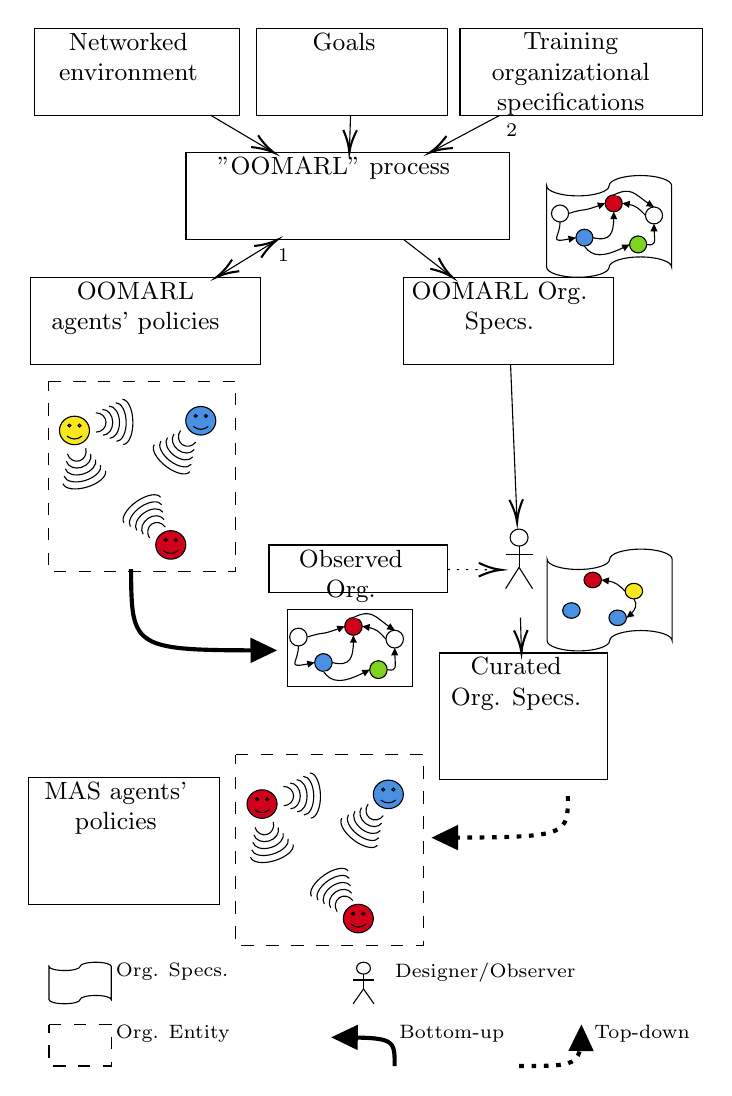
\begin{tikzpicture}[x=0.75pt,y=0.75pt,yscale=-1,xscale=1]
%uncomment if require: \path (0,567); %set diagram left start at 0, and has height of 567

%Flowchart: Punched Tape [id:dp6253416173354658] 
\draw  [fill={rgb, 255:red, 255; green, 255; blue, 255 }  ,fill opacity=1 ] (250,275.87) .. controls (250,278.58) and (256.74,280.77) .. (265.06,280.77) .. controls (273.38,280.77) and (280.12,278.58) .. (280.12,275.87) .. controls (280.12,273.16) and (286.87,270.97) .. (295.18,270.97) .. controls (303.5,270.97) and (310.25,273.16) .. (310.25,275.87) -- (310.25,315.1) .. controls (310.25,312.39) and (303.5,310.19) .. (295.18,310.19) .. controls (286.87,310.19) and (280.12,312.39) .. (280.12,315.1) .. controls (280.12,317.8) and (273.38,320) .. (265.06,320) .. controls (256.74,320) and (250,317.8) .. (250,315.1) -- cycle ;
%Shape: Ellipse [id:dp3141849675822821] 
\draw  [fill={rgb, 255:red, 208; green, 2; blue, 27 }  ,fill opacity=1 ] (267.77,285.83) .. controls (267.77,283.76) and (269.66,282.08) .. (271.98,282.08) .. controls (274.3,282.08) and (276.19,283.76) .. (276.19,285.83) .. controls (276.19,287.9) and (274.3,289.58) .. (271.98,289.58) .. controls (269.66,289.58) and (267.77,287.9) .. (267.77,285.83) -- cycle ;
%Shape: Ellipse [id:dp24618456488955864] 
\draw  [fill={rgb, 255:red, 248; green, 231; blue, 28 }  ,fill opacity=1 ] (287.6,291.19) .. controls (287.6,289.12) and (289.49,287.44) .. (291.81,287.44) .. controls (294.13,287.44) and (296.02,289.12) .. (296.02,291.19) .. controls (296.02,293.27) and (294.13,294.95) .. (291.81,294.95) .. controls (289.49,294.95) and (287.6,293.27) .. (287.6,291.19) -- cycle ;
%Shape: Ellipse [id:dp8783844186516785] 
\draw  [fill={rgb, 255:red, 74; green, 144; blue, 226 }  ,fill opacity=1 ] (279.79,304.06) .. controls (279.79,301.99) and (281.67,300.31) .. (284,300.31) .. controls (286.32,300.31) and (288.2,301.99) .. (288.2,304.06) .. controls (288.2,306.13) and (286.32,307.81) .. (284,307.81) .. controls (281.67,307.81) and (279.79,306.13) .. (279.79,304.06) -- cycle ;
%Curve Lines [id:da8862512396754962] 
\draw [fill={rgb, 255:red, 255; green, 255; blue, 255 }  ,fill opacity=1 ]   (287.6,291.19) .. controls (284.11,287.9) and (283.1,286.97) .. (279.08,286.26) ;
\draw [shift={(276.19,285.83)}, rotate = 7.39] [fill={rgb, 255:red, 0; green, 0; blue, 0 }  ][line width=0.08]  [draw opacity=0] (3.57,-1.72) -- (0,0) -- (3.57,1.72) -- cycle    ;
%Shape: Ellipse [id:dp10865415349748586] 
\draw  [fill={rgb, 255:red, 74; green, 144; blue, 226 }  ,fill opacity=1 ] (257.5,300.55) .. controls (257.5,298.48) and (259.38,296.8) .. (261.71,296.8) .. controls (264.03,296.8) and (265.91,298.48) .. (265.91,300.55) .. controls (265.91,302.62) and (264.03,304.3) .. (261.71,304.3) .. controls (259.38,304.3) and (257.5,302.62) .. (257.5,300.55) -- cycle ;
%Curve Lines [id:da9209146587835657] 
\draw [fill={rgb, 255:red, 255; green, 255; blue, 255 }  ,fill opacity=1 ]   (291.81,294.95) .. controls (293.69,297.65) and (292.57,300.02) .. (290.45,302.13) ;
\draw [shift={(288.2,304.06)}, rotate = 322.38] [fill={rgb, 255:red, 0; green, 0; blue, 0 }  ][line width=0.08]  [draw opacity=0] (3.57,-1.72) -- (0,0) -- (3.57,1.72) -- cycle    ;

%Shape: Rectangle [id:dp5799704037482001] 
\draw  [dash pattern={on 4.5pt off 4.5pt}] (9.63,190) -- (100,190) -- (100,281.94) -- (9.63,281.94) -- cycle ;
%Shape: Smiley Face [id:dp642715493380654] 
\draw  [fill={rgb, 255:red, 248; green, 231; blue, 28 }  ,fill opacity=1 ] (15.05,213.78) .. controls (15.05,209.99) and (18.29,206.92) .. (22.28,206.92) .. controls (26.28,206.92) and (29.51,209.99) .. (29.51,213.78) .. controls (29.51,217.57) and (26.28,220.65) .. (22.28,220.65) .. controls (18.29,220.65) and (15.05,217.57) .. (15.05,213.78) -- cycle ; \draw  [fill={rgb, 255:red, 248; green, 231; blue, 28 }  ,fill opacity=1 ] (19.1,211.45) .. controls (19.1,211.07) and (19.43,210.76) .. (19.82,210.76) .. controls (20.22,210.76) and (20.55,211.07) .. (20.55,211.45) .. controls (20.55,211.83) and (20.22,212.13) .. (19.82,212.13) .. controls (19.43,212.13) and (19.1,211.83) .. (19.1,211.45) -- cycle ; \draw  [fill={rgb, 255:red, 248; green, 231; blue, 28 }  ,fill opacity=1 ] (24.02,211.45) .. controls (24.02,211.07) and (24.34,210.76) .. (24.74,210.76) .. controls (25.14,210.76) and (25.46,211.07) .. (25.46,211.45) .. controls (25.46,211.83) and (25.14,212.13) .. (24.74,212.13) .. controls (24.34,212.13) and (24.02,211.83) .. (24.02,211.45) -- cycle ; \draw   (18.67,216.53) .. controls (21.08,218.36) and (23.49,218.36) .. (25.9,216.53) ;
%Shape: Arc [id:dp7103754459108031] 
\draw  [draw opacity=0] (37.24,233.21) .. controls (37.24,233.21) and (37.24,233.21) .. (37.24,233.21) .. controls (38,235.82) and (34.04,239.33) .. (28.39,241.04) .. controls (22.74,242.76) and (17.53,242.04) .. (16.77,239.43) -- (27,236.32) -- cycle ; \draw   (37.24,233.21) .. controls (37.24,233.21) and (37.24,233.21) .. (37.24,233.21) .. controls (38,235.82) and (34.04,239.33) .. (28.39,241.04) .. controls (22.74,242.76) and (17.53,242.04) .. (16.77,239.43) ;  
%Shape: Arc [id:dp9993647702991559] 
\draw  [draw opacity=0] (34.85,230.5) .. controls (35.62,233.11) and (32.31,236.42) .. (27.46,237.89) .. controls (22.62,239.37) and (18.07,238.44) .. (17.3,235.83) -- (26.08,233.17) -- cycle ; \draw   (34.85,230.5) .. controls (35.62,233.11) and (32.31,236.42) .. (27.46,237.89) .. controls (22.62,239.37) and (18.07,238.44) .. (17.3,235.83) ;  
%Shape: Arc [id:dp33021260729129986] 
\draw  [draw opacity=0] (32.46,227.79) .. controls (32.46,227.79) and (32.46,227.79) .. (32.46,227.79) .. controls (32.46,227.79) and (32.46,227.79) .. (32.46,227.79) .. controls (33.23,230.4) and (30.58,233.51) .. (26.54,234.74) .. controls (22.5,235.97) and (18.61,234.85) .. (17.84,232.24) -- (25.15,230.02) -- cycle ; \draw   (32.46,227.79) .. controls (32.46,227.79) and (32.46,227.79) .. (32.46,227.79) .. controls (32.46,227.79) and (32.46,227.79) .. (32.46,227.79) .. controls (33.23,230.4) and (30.58,233.51) .. (26.54,234.74) .. controls (22.5,235.97) and (18.61,234.85) .. (17.84,232.24) ;  
%Shape: Arc [id:dp7515950702187679] 
\draw  [draw opacity=0] (30.07,225.09) .. controls (30.07,225.09) and (30.07,225.09) .. (30.07,225.09) .. controls (30.07,225.09) and (30.07,225.09) .. (30.07,225.09) .. controls (30.84,227.7) and (28.84,230.61) .. (25.61,231.59) .. controls (22.38,232.57) and (19.14,231.25) .. (18.38,228.64) -- (24.22,226.86) -- cycle ; \draw   (30.07,225.09) .. controls (30.07,225.09) and (30.07,225.09) .. (30.07,225.09) .. controls (30.07,225.09) and (30.07,225.09) .. (30.07,225.09) .. controls (30.84,227.7) and (28.84,230.61) .. (25.61,231.59) .. controls (22.38,232.57) and (19.14,231.25) .. (18.38,228.64) ;  
%Shape: Arc [id:dp17995425823285305] 
\draw  [draw opacity=0] (27.69,222.38) .. controls (27.69,222.38) and (27.69,222.38) .. (27.69,222.38) .. controls (27.69,222.38) and (27.69,222.38) .. (27.69,222.38) .. controls (28.45,224.99) and (27.11,227.7) .. (24.69,228.44) .. controls (22.27,229.18) and (19.68,227.66) .. (18.91,225.05) -- (23.3,223.71) -- cycle ; \draw   (27.69,222.38) .. controls (27.69,222.38) and (27.69,222.38) .. (27.69,222.38) .. controls (27.69,222.38) and (27.69,222.38) .. (27.69,222.38) .. controls (28.45,224.99) and (27.11,227.7) .. (24.69,228.44) .. controls (22.27,229.18) and (19.68,227.66) .. (18.91,225.05) ;  

%Shape: Arc [id:dp8934563741256025] 
\draw  [draw opacity=0] (45.36,198.82) .. controls (48.04,198.76) and (50.3,203.58) .. (50.42,209.59) .. controls (50.54,215.59) and (48.46,220.49) .. (45.78,220.55) -- (45.57,209.68) -- cycle ; \draw   (45.36,198.82) .. controls (48.04,198.76) and (50.3,203.58) .. (50.42,209.59) .. controls (50.54,215.59) and (48.46,220.49) .. (45.78,220.55) ;  
%Shape: Arc [id:dp5963815446588989] 
\draw  [draw opacity=0] (42.16,200.43) .. controls (44.84,200.38) and (47.09,204.51) .. (47.19,209.65) .. controls (47.29,214.79) and (45.2,219.01) .. (42.52,219.06) -- (42.34,209.75) -- cycle ; \draw   (42.16,200.43) .. controls (44.84,200.38) and (47.09,204.51) .. (47.19,209.65) .. controls (47.29,214.79) and (45.2,219.01) .. (42.52,219.06) ;  
%Shape: Arc [id:dp3378668028957823] 
\draw  [draw opacity=0] (38.96,202.05) .. controls (38.96,202.05) and (38.96,202.05) .. (38.96,202.05) .. controls (38.96,202.05) and (38.96,202.05) .. (38.96,202.05) .. controls (41.63,202) and (43.87,205.43) .. (43.96,209.71) .. controls (44.04,214) and (41.94,217.52) .. (39.26,217.57) -- (39.11,209.81) -- cycle ; \draw   (38.96,202.05) .. controls (38.96,202.05) and (38.96,202.05) .. (38.96,202.05) .. controls (38.96,202.05) and (38.96,202.05) .. (38.96,202.05) .. controls (41.63,202) and (43.87,205.43) .. (43.96,209.71) .. controls (44.04,214) and (41.94,217.52) .. (39.26,217.57) ;  
%Shape: Arc [id:dp7870035207223711] 
\draw  [draw opacity=0] (35.76,203.67) .. controls (38.43,203.61) and (40.66,206.35) .. (40.72,209.78) .. controls (40.79,213.21) and (38.67,216.03) .. (36,216.09) -- (35.88,209.88) -- cycle ; \draw   (35.76,203.67) .. controls (38.43,203.61) and (40.66,206.35) .. (40.72,209.78) .. controls (40.79,213.21) and (38.67,216.03) .. (36,216.09) ;  
%Shape: Arc [id:dp7731275981870975] 
\draw  [draw opacity=0] (32.55,205.29) .. controls (32.55,205.29) and (32.55,205.29) .. (32.55,205.29) .. controls (35.23,205.23) and (37.44,207.27) .. (37.49,209.84) .. controls (37.54,212.42) and (35.41,214.54) .. (32.73,214.6) -- (32.64,209.94) -- cycle ; \draw   (32.55,205.29) .. controls (32.55,205.29) and (32.55,205.29) .. (32.55,205.29) .. controls (35.23,205.23) and (37.44,207.27) .. (37.49,209.84) .. controls (37.54,212.42) and (35.41,214.54) .. (32.73,214.6) ;  

%Shape: Smiley Face [id:dp8522771230099253] 
\draw  [fill={rgb, 255:red, 208; green, 2; blue, 27 }  ,fill opacity=1 ] (61.44,268.94) .. controls (61.44,265.15) and (64.68,262.08) .. (68.67,262.08) .. controls (72.66,262.08) and (75.9,265.15) .. (75.9,268.94) .. controls (75.9,272.73) and (72.66,275.81) .. (68.67,275.81) .. controls (64.68,275.81) and (61.44,272.73) .. (61.44,268.94) -- cycle ; \draw  [fill={rgb, 255:red, 208; green, 2; blue, 27 }  ,fill opacity=1 ] (65.49,266.61) .. controls (65.49,266.23) and (65.81,265.92) .. (66.21,265.92) .. controls (66.61,265.92) and (66.94,266.23) .. (66.94,266.61) .. controls (66.94,266.99) and (66.61,267.29) .. (66.21,267.29) .. controls (65.81,267.29) and (65.49,266.99) .. (65.49,266.61) -- cycle ; \draw  [fill={rgb, 255:red, 208; green, 2; blue, 27 }  ,fill opacity=1 ] (70.41,266.61) .. controls (70.41,266.23) and (70.73,265.92) .. (71.13,265.92) .. controls (71.53,265.92) and (71.85,266.23) .. (71.85,266.61) .. controls (71.85,266.99) and (71.53,267.29) .. (71.13,267.29) .. controls (70.73,267.29) and (70.41,266.99) .. (70.41,266.61) -- cycle ; \draw   (65.06,271.69) .. controls (67.47,273.52) and (69.88,273.52) .. (72.29,271.69) ;
%Shape: Arc [id:dp2662505393390908] 
\draw  [draw opacity=0] (46.11,258.27) .. controls (46.11,258.27) and (46.11,258.27) .. (46.11,258.27) .. controls (46.11,258.27) and (46.11,258.27) .. (46.11,258.27) .. controls (44.6,256.02) and (47.31,251.45) .. (52.18,248.06) .. controls (57.04,244.66) and (62.22,243.73) .. (63.73,245.98) -- (54.92,252.13) -- cycle ; \draw   (46.11,258.27) .. controls (46.11,258.27) and (46.11,258.27) .. (46.11,258.27) .. controls (46.11,258.27) and (46.11,258.27) .. (46.11,258.27) .. controls (44.6,256.02) and (47.31,251.45) .. (52.18,248.06) .. controls (57.04,244.66) and (62.22,243.73) .. (63.73,245.98) ;  
%Shape: Arc [id:dp5533657200850002] 
\draw  [draw opacity=0] (49.2,260.11) .. controls (49.2,260.11) and (49.2,260.11) .. (49.2,260.11) .. controls (47.68,257.86) and (49.84,253.68) .. (54.01,250.77) .. controls (58.18,247.86) and (62.79,247.32) .. (64.3,249.57) -- (56.75,254.84) -- cycle ; \draw   (49.2,260.11) .. controls (49.2,260.11) and (49.2,260.11) .. (49.2,260.11) .. controls (47.68,257.86) and (49.84,253.68) .. (54.01,250.77) .. controls (58.18,247.86) and (62.79,247.32) .. (64.3,249.57) ;  
%Shape: Arc [id:dp130720604660594] 
\draw  [draw opacity=0] (52.28,261.94) .. controls (50.77,259.69) and (52.36,255.91) .. (55.84,253.48) .. controls (59.31,251.06) and (63.36,250.91) .. (64.87,253.16) -- (58.58,257.55) -- cycle ; \draw   (52.28,261.94) .. controls (50.77,259.69) and (52.36,255.91) .. (55.84,253.48) .. controls (59.31,251.06) and (63.36,250.91) .. (64.87,253.16) ;  
%Shape: Arc [id:dp7777326608896638] 
\draw  [draw opacity=0] (55.37,263.77) .. controls (55.37,263.77) and (55.37,263.77) .. (55.37,263.77) .. controls (53.86,261.53) and (54.88,258.13) .. (57.66,256.19) .. controls (60.44,254.25) and (63.93,254.5) .. (65.44,256.75) -- (60.41,260.26) -- cycle ; \draw   (55.37,263.77) .. controls (55.37,263.77) and (55.37,263.77) .. (55.37,263.77) .. controls (53.86,261.53) and (54.88,258.13) .. (57.66,256.19) .. controls (60.44,254.25) and (63.93,254.5) .. (65.44,256.75) ;  
%Shape: Arc [id:dp4348101062357661] 
\draw  [draw opacity=0] (58.46,265.61) .. controls (56.94,263.36) and (57.41,260.36) .. (59.49,258.91) .. controls (61.58,257.45) and (64.49,258.09) .. (66.01,260.34) -- (62.23,262.98) -- cycle ; \draw   (58.46,265.61) .. controls (56.94,263.36) and (57.41,260.36) .. (59.49,258.91) .. controls (61.58,257.45) and (64.49,258.09) .. (66.01,260.34) ;  

%Shape: Smiley Face [id:dp8996964185972032] 
\draw  [fill={rgb, 255:red, 74; green, 144; blue, 226 }  ,fill opacity=1 ] (75.9,209.12) .. controls (75.9,205.33) and (79.14,202.26) .. (83.13,202.26) .. controls (87.12,202.26) and (90.36,205.33) .. (90.36,209.12) .. controls (90.36,212.91) and (87.12,215.99) .. (83.13,215.99) .. controls (79.14,215.99) and (75.9,212.91) .. (75.9,209.12) -- cycle ; \draw  [fill={rgb, 255:red, 74; green, 144; blue, 226 }  ,fill opacity=1 ] (79.95,206.79) .. controls (79.95,206.41) and (80.27,206.1) .. (80.67,206.1) .. controls (81.07,206.1) and (81.4,206.41) .. (81.4,206.79) .. controls (81.4,207.17) and (81.07,207.48) .. (80.67,207.48) .. controls (80.27,207.48) and (79.95,207.17) .. (79.95,206.79) -- cycle ; \draw  [fill={rgb, 255:red, 74; green, 144; blue, 226 }  ,fill opacity=1 ] (84.87,206.79) .. controls (84.87,206.41) and (85.19,206.1) .. (85.59,206.1) .. controls (85.99,206.1) and (86.31,206.41) .. (86.31,206.79) .. controls (86.31,207.17) and (85.99,207.48) .. (85.59,207.48) .. controls (85.19,207.48) and (84.87,207.17) .. (84.87,206.79) -- cycle ; \draw   (79.52,211.87) .. controls (81.93,213.7) and (84.34,213.7) .. (86.75,211.87) ;
%Shape: Arc [id:dp6344973920370733] 
\draw  [draw opacity=0] (77.83,233.64) .. controls (77.83,233.64) and (77.83,233.64) .. (77.83,233.64) .. controls (76.23,235.82) and (71.1,234.67) .. (66.38,231.07) .. controls (61.66,227.47) and (59.13,222.79) .. (60.74,220.61) -- (69.28,227.13) -- cycle ; \draw   (77.83,233.64) .. controls (77.83,233.64) and (77.83,233.64) .. (77.83,233.64) .. controls (76.23,235.82) and (71.1,234.67) .. (66.38,231.07) .. controls (61.66,227.47) and (59.13,222.79) .. (60.74,220.61) ;  
%Shape: Arc [id:dp2502725185770005] 
\draw  [draw opacity=0] (78.55,230.08) .. controls (78.55,230.08) and (78.55,230.08) .. (78.55,230.08) .. controls (78.55,230.08) and (78.55,230.08) .. (78.55,230.08) .. controls (76.94,232.26) and (72.36,231.53) .. (68.31,228.44) .. controls (64.27,225.36) and (62.29,221.09) .. (63.9,218.91) -- (71.22,224.49) -- cycle ; \draw   (78.55,230.08) .. controls (78.55,230.08) and (78.55,230.08) .. (78.55,230.08) .. controls (78.55,230.08) and (78.55,230.08) .. (78.55,230.08) .. controls (76.94,232.26) and (72.36,231.53) .. (68.31,228.44) .. controls (64.27,225.36) and (62.29,221.09) .. (63.9,218.91) ;  
%Shape: Arc [id:dp23421846029392612] 
\draw  [draw opacity=0] (79.27,226.52) .. controls (79.27,226.52) and (79.27,226.52) .. (79.27,226.52) .. controls (79.27,226.52) and (79.27,226.52) .. (79.27,226.52) .. controls (77.66,228.7) and (73.63,228.38) .. (70.25,225.81) .. controls (66.88,223.24) and (65.45,219.39) .. (67.06,217.21) -- (73.16,221.86) -- cycle ; \draw   (79.27,226.52) .. controls (79.27,226.52) and (79.27,226.52) .. (79.27,226.52) .. controls (79.27,226.52) and (79.27,226.52) .. (79.27,226.52) .. controls (77.66,228.7) and (73.63,228.38) .. (70.25,225.81) .. controls (66.88,223.24) and (65.45,219.39) .. (67.06,217.21) ;  
%Shape: Arc [id:dp02946644855410807] 
\draw  [draw opacity=0] (79.98,222.95) .. controls (78.38,225.13) and (74.89,225.23) .. (72.19,223.18) .. controls (69.49,221.12) and (68.61,217.69) .. (70.22,215.51) -- (75.1,219.23) -- cycle ; \draw   (79.98,222.95) .. controls (78.38,225.13) and (74.89,225.23) .. (72.19,223.18) .. controls (69.49,221.12) and (68.61,217.69) .. (70.22,215.51) ;  
%Shape: Arc [id:dp07919277634076938] 
\draw  [draw opacity=0] (80.7,219.39) .. controls (80.7,219.39) and (80.7,219.39) .. (80.7,219.39) .. controls (79.1,221.57) and (76.15,222.09) .. (74.13,220.55) .. controls (72.11,219) and (71.77,215.99) .. (73.38,213.81) -- (77.04,216.6) -- cycle ; \draw   (80.7,219.39) .. controls (80.7,219.39) and (80.7,219.39) .. (80.7,219.39) .. controls (79.1,221.57) and (76.15,222.09) .. (74.13,220.55) .. controls (72.11,219) and (71.77,215.99) .. (73.38,213.81) ;  

%Flowchart: Punched Tape [id:dp1596519476860545] 
\draw  [fill={rgb, 255:red, 255; green, 255; blue, 255 }  ,fill opacity=1 ] (249.75,95.87) .. controls (249.75,98.58) and (256.5,100.77) .. (264.82,100.77) .. controls (273.13,100.77) and (279.88,98.58) .. (279.88,95.87) .. controls (279.88,93.16) and (286.62,90.97) .. (294.94,90.97) .. controls (303.26,90.97) and (310,93.16) .. (310,95.87) -- (310,135.1) .. controls (310,132.39) and (303.26,130.19) .. (294.94,130.19) .. controls (286.62,130.19) and (279.88,132.39) .. (279.88,135.1) .. controls (279.88,137.8) and (273.13,140) .. (264.82,140) .. controls (256.5,140) and (249.75,137.8) .. (249.75,135.1) -- cycle ;
%Shape: Ellipse [id:dp002685494295735058] 
\draw  [fill={rgb, 255:red, 255; green, 255; blue, 255 }  ,fill opacity=1 ] (252.11,109.26) .. controls (252.11,107.01) and (253.95,105.18) .. (256.22,105.18) .. controls (258.5,105.18) and (260.34,107.01) .. (260.34,109.26) .. controls (260.34,111.51) and (258.5,113.33) .. (256.22,113.33) .. controls (253.95,113.33) and (252.11,111.51) .. (252.11,109.26) -- cycle ;
%Shape: Ellipse [id:dp18321883985201803] 
\draw  [fill={rgb, 255:red, 74; green, 144; blue, 226 }  ,fill opacity=1 ] (263.87,120.91) .. controls (263.87,118.65) and (265.71,116.83) .. (267.98,116.83) .. controls (270.26,116.83) and (272.1,118.65) .. (272.1,120.91) .. controls (272.1,123.16) and (270.26,124.98) .. (267.98,124.98) .. controls (265.71,124.98) and (263.87,123.16) .. (263.87,120.91) -- cycle ;
%Shape: Ellipse [id:dp4076602785297232] 
\draw  [fill={rgb, 255:red, 208; green, 2; blue, 27 }  ,fill opacity=1 ] (277.98,104.36) .. controls (277.98,102.11) and (279.82,100.29) .. (282.1,100.29) .. controls (284.37,100.29) and (286.21,102.11) .. (286.21,104.36) .. controls (286.21,106.62) and (284.37,108.44) .. (282.1,108.44) .. controls (279.82,108.44) and (277.98,106.62) .. (277.98,104.36) -- cycle ;
%Shape: Ellipse [id:dp9213295790384606] 
\draw  [fill={rgb, 255:red, 255; green, 255; blue, 255 }  ,fill opacity=1 ] (297.38,110.19) .. controls (297.38,107.94) and (299.23,106.11) .. (301.5,106.11) .. controls (303.77,106.11) and (305.62,107.94) .. (305.62,110.19) .. controls (305.62,112.44) and (303.77,114.27) .. (301.5,114.27) .. controls (299.23,114.27) and (297.38,112.44) .. (297.38,110.19) -- cycle ;
%Shape: Ellipse [id:dp07303077783269196] 
\draw  [fill={rgb, 255:red, 126; green, 211; blue, 33 }  ,fill opacity=1 ] (289.74,124.17) .. controls (289.74,121.92) and (291.58,120.09) .. (293.86,120.09) .. controls (296.13,120.09) and (297.97,121.92) .. (297.97,124.17) .. controls (297.97,126.42) and (296.13,128.24) .. (293.86,128.24) .. controls (291.58,128.24) and (289.74,126.42) .. (289.74,124.17) -- cycle ;
%Curve Lines [id:da40084119138850793] 
\draw [fill={rgb, 255:red, 255; green, 255; blue, 255 }  ,fill opacity=1 ]   (260.34,109.26) .. controls (269.59,106.35) and (265.25,108.92) .. (275.25,105.36) ;
\draw [shift={(277.98,104.36)}, rotate = 159.68] [fill={rgb, 255:red, 0; green, 0; blue, 0 }  ][line width=0.08]  [draw opacity=0] (3.57,-1.72) -- (0,0) -- (3.57,1.72) -- cycle    ;
%Curve Lines [id:da056316075040988345] 
\draw [fill={rgb, 255:red, 255; green, 255; blue, 255 }  ,fill opacity=1 ]   (272.1,120.91) .. controls (280.9,123.06) and (281.95,118.36) .. (282.08,111.4) ;
\draw [shift={(282.1,108.44)}, rotate = 90] [fill={rgb, 255:red, 0; green, 0; blue, 0 }  ][line width=0.08]  [draw opacity=0] (3.57,-1.72) -- (0,0) -- (3.57,1.72) -- cycle    ;
%Curve Lines [id:da9750985583942122] 
\draw [fill={rgb, 255:red, 255; green, 255; blue, 255 }  ,fill opacity=1 ]   (297.38,110.19) .. controls (293.99,106.63) and (292.99,105.61) .. (289.12,104.84) ;
\draw [shift={(286.21,104.36)}, rotate = 8.2] [fill={rgb, 255:red, 0; green, 0; blue, 0 }  ][line width=0.08]  [draw opacity=0] (3.57,-1.72) -- (0,0) -- (3.57,1.72) -- cycle    ;
%Curve Lines [id:da6143174667543494] 
\draw [fill={rgb, 255:red, 255; green, 255; blue, 255 }  ,fill opacity=1 ]   (297.97,124.17) .. controls (302.6,124.98) and (301.83,123.3) .. (301.57,117.17) ;
\draw [shift={(301.5,114.27)}, rotate = 90] [fill={rgb, 255:red, 0; green, 0; blue, 0 }  ][line width=0.08]  [draw opacity=0] (3.57,-1.72) -- (0,0) -- (3.57,1.72) -- cycle    ;
%Curve Lines [id:da2385044516658259] 
\draw [fill={rgb, 255:red, 255; green, 255; blue, 255 }  ,fill opacity=1 ]   (256.22,113.33) .. controls (256.22,121.03) and (250.12,123.58) .. (261.09,121.46) ;
\draw [shift={(263.87,120.91)}, rotate = 168.36] [fill={rgb, 255:red, 0; green, 0; blue, 0 }  ][line width=0.08]  [draw opacity=0] (3.57,-1.72) -- (0,0) -- (3.57,1.72) -- cycle    ;
%Curve Lines [id:da43759757255400467] 
\draw [fill={rgb, 255:red, 255; green, 255; blue, 255 }  ,fill opacity=1 ]   (267.98,124.98) .. controls (271.79,130.48) and (277.11,130.39) .. (287.19,125.46) ;
\draw [shift={(289.74,124.17)}, rotate = 152.3] [fill={rgb, 255:red, 0; green, 0; blue, 0 }  ][line width=0.08]  [draw opacity=0] (3.57,-1.72) -- (0,0) -- (3.57,1.72) -- cycle    ;
%Curve Lines [id:da6953413668483659] 
\draw [fill={rgb, 255:red, 255; green, 255; blue, 255 }  ,fill opacity=1 ]   (282.1,100.29) .. controls (290.61,96.28) and (291.9,99.72) .. (299.04,104.55) ;
\draw [shift={(301.5,106.11)}, rotate = 210.72] [fill={rgb, 255:red, 0; green, 0; blue, 0 }  ][line width=0.08]  [draw opacity=0] (3.57,-1.72) -- (0,0) -- (3.57,1.72) -- cycle    ;

%Shape: Ellipse [id:dp5665300419613197] 
\draw   (232.16,265.4) .. controls (232.16,263.14) and (234.1,261.3) .. (236.49,261.3) .. controls (238.88,261.3) and (240.82,263.14) .. (240.82,265.4) .. controls (240.82,267.67) and (238.88,269.5) .. (236.49,269.5) .. controls (234.1,269.5) and (232.16,267.67) .. (232.16,265.4) -- cycle ;
%Straight Lines [id:da868287133321088] 
\draw    (236.49,269.5) -- (236.49,279.75) ;
%Straight Lines [id:da7338999456859931] 
\draw    (236.49,279.75) -- (230,290) ;
%Straight Lines [id:da7618645013452761] 
\draw    (236.49,279.75) -- (242.98,290) ;
%Straight Lines [id:da7029210082761028] 
\draw    (242.98,273.6) -- (230,273.6) ;

%Shape: Rectangle [id:dp36259598060414655] 
\draw  [fill={rgb, 255:red, 255; green, 255; blue, 255 }  ,fill opacity=1 ] (124.75,300.23) -- (185,300.23) -- (185,337) -- (124.75,337) -- cycle ;
%Shape: Ellipse [id:dp34598635042601256] 
\draw  [fill={rgb, 255:red, 255; green, 255; blue, 255 }  ,fill opacity=1 ] (125.96,313.34) .. controls (125.96,310.97) and (127.85,309.05) .. (130.18,309.05) .. controls (132.51,309.05) and (134.39,310.97) .. (134.39,313.34) .. controls (134.39,315.71) and (132.51,317.63) .. (130.18,317.63) .. controls (127.85,317.63) and (125.96,315.71) .. (125.96,313.34) -- cycle ;
%Shape: Ellipse [id:dp0011247415244253212] 
\draw  [fill={rgb, 255:red, 74; green, 144; blue, 226 }  ,fill opacity=1 ] (138.01,325.6) .. controls (138.01,323.23) and (139.9,321.31) .. (142.23,321.31) .. controls (144.55,321.31) and (146.44,323.23) .. (146.44,325.6) .. controls (146.44,327.97) and (144.55,329.89) .. (142.23,329.89) .. controls (139.9,329.89) and (138.01,327.97) .. (138.01,325.6) -- cycle ;
%Shape: Ellipse [id:dp8822927144483022] 
\draw  [fill={rgb, 255:red, 208; green, 2; blue, 27 }  ,fill opacity=1 ] (152.47,308.19) .. controls (152.47,305.82) and (154.36,303.9) .. (156.68,303.9) .. controls (159.01,303.9) and (160.9,305.82) .. (160.9,308.19) .. controls (160.9,310.56) and (159.01,312.48) .. (156.68,312.48) .. controls (154.36,312.48) and (152.47,310.56) .. (152.47,308.19) -- cycle ;
%Shape: Ellipse [id:dp7611446545020739] 
\draw  [fill={rgb, 255:red, 255; green, 255; blue, 255 }  ,fill opacity=1 ] (172.35,314.32) .. controls (172.35,311.95) and (174.24,310.03) .. (176.57,310.03) .. controls (178.89,310.03) and (180.78,311.95) .. (180.78,314.32) .. controls (180.78,316.69) and (178.89,318.61) .. (176.57,318.61) .. controls (174.24,318.61) and (172.35,316.69) .. (172.35,314.32) -- cycle ;
%Shape: Ellipse [id:dp1592826898001829] 
\draw  [fill={rgb, 255:red, 126; green, 211; blue, 33 }  ,fill opacity=1 ] (164.52,329.03) .. controls (164.52,326.66) and (166.4,324.74) .. (168.73,324.74) .. controls (171.06,324.74) and (172.95,326.66) .. (172.95,329.03) .. controls (172.95,331.4) and (171.06,333.32) .. (168.73,333.32) .. controls (166.4,333.32) and (164.52,331.4) .. (164.52,329.03) -- cycle ;
%Curve Lines [id:da27399536046205264] 
\draw [fill={rgb, 255:red, 255; green, 255; blue, 255 }  ,fill opacity=1 ]   (134.39,313.34) .. controls (143.87,310.28) and (139.42,312.99) .. (149.67,309.24) ;
\draw [shift={(152.47,308.19)}, rotate = 159.17] [fill={rgb, 255:red, 0; green, 0; blue, 0 }  ][line width=0.08]  [draw opacity=0] (3.57,-1.72) -- (0,0) -- (3.57,1.72) -- cycle    ;
%Curve Lines [id:da16623917428090795] 
\draw [fill={rgb, 255:red, 255; green, 255; blue, 255 }  ,fill opacity=1 ]   (146.44,325.6) .. controls (155.51,327.88) and (156.55,322.86) .. (156.67,315.47) ;
\draw [shift={(156.68,312.48)}, rotate = 90] [fill={rgb, 255:red, 0; green, 0; blue, 0 }  ][line width=0.08]  [draw opacity=0] (3.57,-1.72) -- (0,0) -- (3.57,1.72) -- cycle    ;
%Curve Lines [id:da46234775845087284] 
\draw [fill={rgb, 255:red, 255; green, 255; blue, 255 }  ,fill opacity=1 ]   (172.35,314.32) .. controls (168.85,310.56) and (167.84,309.5) .. (163.81,308.68) ;
\draw [shift={(160.9,308.19)}, rotate = 8.42] [fill={rgb, 255:red, 0; green, 0; blue, 0 }  ][line width=0.08]  [draw opacity=0] (3.57,-1.72) -- (0,0) -- (3.57,1.72) -- cycle    ;
%Curve Lines [id:da3119386523209393] 
\draw [fill={rgb, 255:red, 255; green, 255; blue, 255 }  ,fill opacity=1 ]   (172.95,329.03) .. controls (177.72,329.9) and (176.9,328.1) .. (176.63,321.56) ;
\draw [shift={(176.57,318.61)}, rotate = 90] [fill={rgb, 255:red, 0; green, 0; blue, 0 }  ][line width=0.08]  [draw opacity=0] (3.57,-1.72) -- (0,0) -- (3.57,1.72) -- cycle    ;
%Curve Lines [id:da8983756138417751] 
\draw [fill={rgb, 255:red, 255; green, 255; blue, 255 }  ,fill opacity=1 ]   (130.18,317.63) .. controls (130.18,325.73) and (123.92,328.41) .. (135.16,326.19) ;
\draw [shift={(138.01,325.6)}, rotate = 168.05] [fill={rgb, 255:red, 0; green, 0; blue, 0 }  ][line width=0.08]  [draw opacity=0] (3.57,-1.72) -- (0,0) -- (3.57,1.72) -- cycle    ;
%Curve Lines [id:da8579733900345894] 
\draw [fill={rgb, 255:red, 255; green, 255; blue, 255 }  ,fill opacity=1 ]   (142.23,329.89) .. controls (146.13,335.67) and (151.57,335.58) .. (161.91,330.39) ;
\draw [shift={(164.52,329.03)}, rotate = 151.67] [fill={rgb, 255:red, 0; green, 0; blue, 0 }  ][line width=0.08]  [draw opacity=0] (3.57,-1.72) -- (0,0) -- (3.57,1.72) -- cycle    ;
%Curve Lines [id:da598997074659714] 
\draw [fill={rgb, 255:red, 255; green, 255; blue, 255 }  ,fill opacity=1 ]   (156.68,303.9) .. controls (165.46,299.66) and (166.74,303.34) .. (174.17,308.47) ;
\draw [shift={(176.57,310.03)}, rotate = 211.4] [fill={rgb, 255:red, 0; green, 0; blue, 0 }  ][line width=0.08]  [draw opacity=0] (3.57,-1.72) -- (0,0) -- (3.57,1.72) -- cycle    ;

%Shape: Boxed Bezier Curve [id:dp053122350641656046] 
\draw [line width=1.5]    (49.54,280.62) .. controls (49.81,319.22) and (49.81,319.8) .. (116.76,319.73) ;
\draw [shift={(119.86,319.73)}, rotate = 179.93] [fill={rgb, 255:red, 0; green, 0; blue, 0 }  ][line width=0.08]  [draw opacity=0] (12.77,-6.13) -- (0,0) -- (12.77,6.13) -- cycle    ;
%Shape: Boxed Bezier Curve [id:dp06305687651907688] 
\draw [line width=1.5]  [dash pattern={on 1.69pt off 2.76pt}]  (260,390) .. controls (260,392.58) and (260,394.82) .. (259.86,396.77) .. controls (258.91,409.54) and (251.75,409.82) .. (197.68,409.99) ;
\draw [shift={(194.31,410)}, rotate = 359.83] [fill={rgb, 255:red, 0; green, 0; blue, 0 }  ][line width=0.08]  [draw opacity=0] (12.77,-6.13) -- (0,0) -- (12.77,6.13) -- cycle    ;
%Shape: Rectangle [id:dp5452427371203186] 
\draw  [dash pattern={on 4.5pt off 4.5pt}] (100,370) -- (190.37,370) -- (190.37,461.94) -- (100,461.94) -- cycle ;
%Shape: Smiley Face [id:dp6068069939037741] 
\draw  [fill={rgb, 255:red, 208; green, 2; blue, 27 }  ,fill opacity=1 ] (105.42,393.78) .. controls (105.42,389.99) and (108.66,386.92) .. (112.65,386.92) .. controls (116.64,386.92) and (119.88,389.99) .. (119.88,393.78) .. controls (119.88,397.57) and (116.64,400.65) .. (112.65,400.65) .. controls (108.66,400.65) and (105.42,397.57) .. (105.42,393.78) -- cycle ; \draw  [fill={rgb, 255:red, 208; green, 2; blue, 27 }  ,fill opacity=1 ] (109.47,391.45) .. controls (109.47,391.07) and (109.79,390.76) .. (110.19,390.76) .. controls (110.59,390.76) and (110.92,391.07) .. (110.92,391.45) .. controls (110.92,391.83) and (110.59,392.13) .. (110.19,392.13) .. controls (109.79,392.13) and (109.47,391.83) .. (109.47,391.45) -- cycle ; \draw  [fill={rgb, 255:red, 208; green, 2; blue, 27 }  ,fill opacity=1 ] (114.39,391.45) .. controls (114.39,391.07) and (114.71,390.76) .. (115.11,390.76) .. controls (115.51,390.76) and (115.83,391.07) .. (115.83,391.45) .. controls (115.83,391.83) and (115.51,392.13) .. (115.11,392.13) .. controls (114.71,392.13) and (114.39,391.83) .. (114.39,391.45) -- cycle ; \draw   (109.04,396.53) .. controls (111.45,398.36) and (113.86,398.36) .. (116.27,396.53) ;
%Shape: Arc [id:dp40222913228483237] 
\draw  [draw opacity=0] (127.61,413.21) .. controls (127.61,413.21) and (127.61,413.21) .. (127.61,413.21) .. controls (128.37,415.82) and (124.41,419.33) .. (118.76,421.04) .. controls (113.11,422.76) and (107.9,422.04) .. (107.14,419.43) -- (117.37,416.32) -- cycle ; \draw   (127.61,413.21) .. controls (127.61,413.21) and (127.61,413.21) .. (127.61,413.21) .. controls (128.37,415.82) and (124.41,419.33) .. (118.76,421.04) .. controls (113.11,422.76) and (107.9,422.04) .. (107.14,419.43) ;  
%Shape: Arc [id:dp6185790641450695] 
\draw  [draw opacity=0] (125.22,410.5) .. controls (125.98,413.11) and (122.68,416.42) .. (117.83,417.89) .. controls (112.99,419.37) and (108.44,418.44) .. (107.67,415.83) -- (116.44,413.17) -- cycle ; \draw   (125.22,410.5) .. controls (125.98,413.11) and (122.68,416.42) .. (117.83,417.89) .. controls (112.99,419.37) and (108.44,418.44) .. (107.67,415.83) ;  
%Shape: Arc [id:dp6749114191148724] 
\draw  [draw opacity=0] (122.83,407.79) .. controls (122.83,407.79) and (122.83,407.79) .. (122.83,407.79) .. controls (123.6,410.4) and (120.95,413.51) .. (116.91,414.74) .. controls (112.87,415.97) and (108.98,414.85) .. (108.21,412.24) -- (115.52,410.02) -- cycle ; \draw   (122.83,407.79) .. controls (122.83,407.79) and (122.83,407.79) .. (122.83,407.79) .. controls (123.6,410.4) and (120.95,413.51) .. (116.91,414.74) .. controls (112.87,415.97) and (108.98,414.85) .. (108.21,412.24) ;  
%Shape: Arc [id:dp056403546095020296] 
\draw  [draw opacity=0] (120.44,405.09) .. controls (120.44,405.09) and (120.44,405.09) .. (120.44,405.09) .. controls (120.44,405.09) and (120.44,405.09) .. (120.44,405.09) .. controls (121.21,407.7) and (119.21,410.61) .. (115.98,411.59) .. controls (112.75,412.57) and (109.51,411.25) .. (108.75,408.64) -- (114.59,406.86) -- cycle ; \draw   (120.44,405.09) .. controls (120.44,405.09) and (120.44,405.09) .. (120.44,405.09) .. controls (120.44,405.09) and (120.44,405.09) .. (120.44,405.09) .. controls (121.21,407.7) and (119.21,410.61) .. (115.98,411.59) .. controls (112.75,412.57) and (109.51,411.25) .. (108.75,408.64) ;  
%Shape: Arc [id:dp048963270262922354] 
\draw  [draw opacity=0] (118.05,402.38) .. controls (118.05,402.38) and (118.05,402.38) .. (118.05,402.38) .. controls (118.82,404.99) and (117.48,407.7) .. (115.06,408.44) .. controls (112.63,409.18) and (110.05,407.66) .. (109.28,405.05) -- (113.67,403.71) -- cycle ; \draw   (118.05,402.38) .. controls (118.05,402.38) and (118.05,402.38) .. (118.05,402.38) .. controls (118.82,404.99) and (117.48,407.7) .. (115.06,408.44) .. controls (112.63,409.18) and (110.05,407.66) .. (109.28,405.05) ;  

%Shape: Arc [id:dp11791815378481285] 
\draw  [draw opacity=0] (135.73,378.82) .. controls (135.73,378.82) and (135.73,378.82) .. (135.73,378.82) .. controls (138.41,378.76) and (140.67,383.58) .. (140.79,389.59) .. controls (140.9,395.59) and (138.83,400.49) .. (136.15,400.55) -- (135.94,389.68) -- cycle ; \draw   (135.73,378.82) .. controls (135.73,378.82) and (135.73,378.82) .. (135.73,378.82) .. controls (138.41,378.76) and (140.67,383.58) .. (140.79,389.59) .. controls (140.9,395.59) and (138.83,400.49) .. (136.15,400.55) ;  
%Shape: Arc [id:dp6186444432706435] 
\draw  [draw opacity=0] (132.53,380.43) .. controls (135.21,380.38) and (137.46,384.51) .. (137.56,389.65) .. controls (137.66,394.79) and (135.57,399.01) .. (132.89,399.06) -- (132.71,389.75) -- cycle ; \draw   (132.53,380.43) .. controls (135.21,380.38) and (137.46,384.51) .. (137.56,389.65) .. controls (137.66,394.79) and (135.57,399.01) .. (132.89,399.06) ;  
%Shape: Arc [id:dp3524256769019909] 
\draw  [draw opacity=0] (129.33,382.05) .. controls (129.33,382.05) and (129.33,382.05) .. (129.33,382.05) .. controls (129.33,382.05) and (129.33,382.05) .. (129.33,382.05) .. controls (132,382) and (134.24,385.43) .. (134.32,389.71) .. controls (134.41,394) and (132.3,397.52) .. (129.63,397.57) .. controls (129.63,397.57) and (129.63,397.57) .. (129.63,397.57) -- (129.48,389.81) -- cycle ; \draw   (129.33,382.05) .. controls (129.33,382.05) and (129.33,382.05) .. (129.33,382.05) .. controls (129.33,382.05) and (129.33,382.05) .. (129.33,382.05) .. controls (132,382) and (134.24,385.43) .. (134.32,389.71) .. controls (134.41,394) and (132.3,397.52) .. (129.63,397.57) .. controls (129.63,397.57) and (129.63,397.57) .. (129.63,397.57) ;  
%Shape: Arc [id:dp9364872182962407] 
\draw  [draw opacity=0] (126.12,383.67) .. controls (128.8,383.61) and (131.03,386.35) .. (131.09,389.78) .. controls (131.16,393.21) and (129.04,396.03) .. (126.36,396.09) -- (126.24,389.88) -- cycle ; \draw   (126.12,383.67) .. controls (128.8,383.61) and (131.03,386.35) .. (131.09,389.78) .. controls (131.16,393.21) and (129.04,396.03) .. (126.36,396.09) ;  
%Shape: Arc [id:dp43568764349824574] 
\draw  [draw opacity=0] (122.92,385.29) .. controls (122.92,385.29) and (122.92,385.29) .. (122.92,385.29) .. controls (125.6,385.23) and (127.81,387.27) .. (127.86,389.84) .. controls (127.91,392.42) and (125.78,394.54) .. (123.1,394.6) -- (123.01,389.94) -- cycle ; \draw   (122.92,385.29) .. controls (122.92,385.29) and (122.92,385.29) .. (122.92,385.29) .. controls (125.6,385.23) and (127.81,387.27) .. (127.86,389.84) .. controls (127.91,392.42) and (125.78,394.54) .. (123.1,394.6) ;  

%Shape: Smiley Face [id:dp7767109991490764] 
\draw  [fill={rgb, 255:red, 208; green, 2; blue, 27 }  ,fill opacity=1 ] (151.81,448.94) .. controls (151.81,445.15) and (155.05,442.08) .. (159.04,442.08) .. controls (163.03,442.08) and (166.27,445.15) .. (166.27,448.94) .. controls (166.27,452.73) and (163.03,455.81) .. (159.04,455.81) .. controls (155.05,455.81) and (151.81,452.73) .. (151.81,448.94) -- cycle ; \draw  [fill={rgb, 255:red, 208; green, 2; blue, 27 }  ,fill opacity=1 ] (155.86,446.61) .. controls (155.86,446.23) and (156.18,445.92) .. (156.58,445.92) .. controls (156.98,445.92) and (157.31,446.23) .. (157.31,446.61) .. controls (157.31,446.99) and (156.98,447.29) .. (156.58,447.29) .. controls (156.18,447.29) and (155.86,446.99) .. (155.86,446.61) -- cycle ; \draw  [fill={rgb, 255:red, 208; green, 2; blue, 27 }  ,fill opacity=1 ] (160.78,446.61) .. controls (160.78,446.23) and (161.1,445.92) .. (161.5,445.92) .. controls (161.9,445.92) and (162.22,446.23) .. (162.22,446.61) .. controls (162.22,446.99) and (161.9,447.29) .. (161.5,447.29) .. controls (161.1,447.29) and (160.78,446.99) .. (160.78,446.61) -- cycle ; \draw   (155.43,451.69) .. controls (157.84,453.52) and (160.25,453.52) .. (162.66,451.69) ;
%Shape: Arc [id:dp12338485660705834] 
\draw  [draw opacity=0] (136.48,438.27) .. controls (136.48,438.27) and (136.48,438.27) .. (136.48,438.27) .. controls (134.97,436.02) and (137.68,431.45) .. (142.55,428.06) .. controls (147.41,424.66) and (152.59,423.73) .. (154.1,425.98) -- (145.29,432.13) -- cycle ; \draw   (136.48,438.27) .. controls (136.48,438.27) and (136.48,438.27) .. (136.48,438.27) .. controls (134.97,436.02) and (137.68,431.45) .. (142.55,428.06) .. controls (147.41,424.66) and (152.59,423.73) .. (154.1,425.98) ;  
%Shape: Arc [id:dp047340824310728946] 
\draw  [draw opacity=0] (139.57,440.11) .. controls (139.57,440.11) and (139.57,440.11) .. (139.57,440.11) .. controls (138.05,437.86) and (140.21,433.68) .. (144.38,430.77) .. controls (148.55,427.86) and (153.15,427.32) .. (154.67,429.57) -- (147.12,434.84) -- cycle ; \draw   (139.57,440.11) .. controls (139.57,440.11) and (139.57,440.11) .. (139.57,440.11) .. controls (138.05,437.86) and (140.21,433.68) .. (144.38,430.77) .. controls (148.55,427.86) and (153.15,427.32) .. (154.67,429.57) ;  
%Shape: Arc [id:dp5460583680593605] 
\draw  [draw opacity=0] (142.65,441.94) .. controls (141.14,439.69) and (142.73,435.91) .. (146.2,433.48) .. controls (149.68,431.06) and (153.72,430.91) .. (155.24,433.16) -- (148.95,437.55) -- cycle ; \draw   (142.65,441.94) .. controls (141.14,439.69) and (142.73,435.91) .. (146.2,433.48) .. controls (149.68,431.06) and (153.72,430.91) .. (155.24,433.16) ;  
%Shape: Arc [id:dp9281425971103023] 
\draw  [draw opacity=0] (145.74,443.77) .. controls (145.74,443.77) and (145.74,443.77) .. (145.74,443.77) .. controls (144.23,441.53) and (145.25,438.13) .. (148.03,436.19) .. controls (150.81,434.25) and (154.29,434.5) .. (155.81,436.75) -- (150.77,440.26) -- cycle ; \draw   (145.74,443.77) .. controls (145.74,443.77) and (145.74,443.77) .. (145.74,443.77) .. controls (144.23,441.53) and (145.25,438.13) .. (148.03,436.19) .. controls (150.81,434.25) and (154.29,434.5) .. (155.81,436.75) ;  
%Shape: Arc [id:dp6708756452099565] 
\draw  [draw opacity=0] (148.83,445.61) .. controls (148.83,445.61) and (148.83,445.61) .. (148.83,445.61) .. controls (147.31,443.36) and (147.78,440.36) .. (149.86,438.91) .. controls (151.95,437.45) and (154.86,438.09) .. (156.38,440.34) -- (152.6,442.98) -- cycle ; \draw   (148.83,445.61) .. controls (148.83,445.61) and (148.83,445.61) .. (148.83,445.61) .. controls (147.31,443.36) and (147.78,440.36) .. (149.86,438.91) .. controls (151.95,437.45) and (154.86,438.09) .. (156.38,440.34) ;  

%Shape: Smiley Face [id:dp23896462419705533] 
\draw  [fill={rgb, 255:red, 74; green, 144; blue, 226 }  ,fill opacity=1 ] (166.27,389.12) .. controls (166.27,385.33) and (169.51,382.26) .. (173.5,382.26) .. controls (177.49,382.26) and (180.73,385.33) .. (180.73,389.12) .. controls (180.73,392.91) and (177.49,395.99) .. (173.5,395.99) .. controls (169.51,395.99) and (166.27,392.91) .. (166.27,389.12) -- cycle ; \draw  [fill={rgb, 255:red, 74; green, 144; blue, 226 }  ,fill opacity=1 ] (170.32,386.79) .. controls (170.32,386.41) and (170.64,386.1) .. (171.04,386.1) .. controls (171.44,386.1) and (171.76,386.41) .. (171.76,386.79) .. controls (171.76,387.17) and (171.44,387.48) .. (171.04,387.48) .. controls (170.64,387.48) and (170.32,387.17) .. (170.32,386.79) -- cycle ; \draw  [fill={rgb, 255:red, 74; green, 144; blue, 226 }  ,fill opacity=1 ] (175.23,386.79) .. controls (175.23,386.41) and (175.56,386.1) .. (175.96,386.1) .. controls (176.36,386.1) and (176.68,386.41) .. (176.68,386.79) .. controls (176.68,387.17) and (176.36,387.48) .. (175.96,387.48) .. controls (175.56,387.48) and (175.23,387.17) .. (175.23,386.79) -- cycle ; \draw   (169.89,391.87) .. controls (172.29,393.7) and (174.7,393.7) .. (177.11,391.87) ;
%Shape: Arc [id:dp8977395703020796] 
\draw  [draw opacity=0] (168.2,413.64) .. controls (168.2,413.64) and (168.2,413.64) .. (168.2,413.64) .. controls (166.6,415.82) and (161.47,414.67) .. (156.74,411.07) .. controls (152.02,407.47) and (149.5,402.79) .. (151.1,400.61) -- (159.65,407.13) -- cycle ; \draw   (168.2,413.64) .. controls (168.2,413.64) and (168.2,413.64) .. (168.2,413.64) .. controls (166.6,415.82) and (161.47,414.67) .. (156.74,411.07) .. controls (152.02,407.47) and (149.5,402.79) .. (151.1,400.61) ;  
%Shape: Arc [id:dp38070292756653834] 
\draw  [draw opacity=0] (168.92,410.08) .. controls (168.92,410.08) and (168.92,410.08) .. (168.92,410.08) .. controls (168.92,410.08) and (168.92,410.08) .. (168.92,410.08) .. controls (167.31,412.26) and (162.73,411.53) .. (158.68,408.44) .. controls (154.64,405.36) and (152.66,401.09) .. (154.26,398.91) -- (161.59,404.49) -- cycle ; \draw   (168.92,410.08) .. controls (168.92,410.08) and (168.92,410.08) .. (168.92,410.08) .. controls (168.92,410.08) and (168.92,410.08) .. (168.92,410.08) .. controls (167.31,412.26) and (162.73,411.53) .. (158.68,408.44) .. controls (154.64,405.36) and (152.66,401.09) .. (154.26,398.91) ;  
%Shape: Arc [id:dp6719893406275441] 
\draw  [draw opacity=0] (169.64,406.52) .. controls (168.03,408.7) and (163.99,408.38) .. (160.62,405.81) .. controls (157.25,403.24) and (155.82,399.39) .. (157.42,397.21) -- (163.53,401.86) -- cycle ; \draw   (169.64,406.52) .. controls (168.03,408.7) and (163.99,408.38) .. (160.62,405.81) .. controls (157.25,403.24) and (155.82,399.39) .. (157.42,397.21) ;  
%Shape: Arc [id:dp8811123580129818] 
\draw  [draw opacity=0] (170.35,402.95) .. controls (168.75,405.13) and (165.26,405.23) .. (162.56,403.18) .. controls (159.86,401.12) and (158.98,397.69) .. (160.58,395.51) -- (165.47,399.23) -- cycle ; \draw   (170.35,402.95) .. controls (168.75,405.13) and (165.26,405.23) .. (162.56,403.18) .. controls (159.86,401.12) and (158.98,397.69) .. (160.58,395.51) ;  
%Shape: Arc [id:dp008168376750506745] 
\draw  [draw opacity=0] (171.07,399.39) .. controls (169.46,401.57) and (166.52,402.09) .. (164.5,400.55) .. controls (162.48,399) and (162.14,395.99) .. (163.74,393.81) -- (167.41,396.6) -- cycle ; \draw   (171.07,399.39) .. controls (169.46,401.57) and (166.52,402.09) .. (164.5,400.55) .. controls (162.48,399) and (162.14,395.99) .. (163.74,393.81) ;  

%Flowchart: Punched Tape [id:dp06290194740685484] 
\draw  [fill={rgb, 255:red, 255; green, 255; blue, 255 }  ,fill opacity=1 ] (10,472) .. controls (10,473.1) and (13.36,474) .. (17.5,474) .. controls (21.64,474) and (25,473.1) .. (25,472) .. controls (25,470.9) and (28.36,470) .. (32.5,470) .. controls (36.64,470) and (40,470.9) .. (40,472) -- (40,488) .. controls (40,486.9) and (36.64,486) .. (32.5,486) .. controls (28.36,486) and (25,486.9) .. (25,488) .. controls (25,489.1) and (21.64,490) .. (17.5,490) .. controls (13.36,490) and (10,489.1) .. (10,488) -- cycle ;
%Shape: Rectangle [id:dp5171976677084227] 
\draw  [dash pattern={on 4.5pt off 4.5pt}] (10,500) -- (40,500) -- (40,520) -- (10,520) -- cycle ;
%Shape: Ellipse [id:dp5593235195310067] 
\draw   (158.21,472.86) .. controls (158.21,471.28) and (159.7,470) .. (161.55,470) .. controls (163.39,470) and (164.88,471.28) .. (164.88,472.86) .. controls (164.88,474.44) and (163.39,475.71) .. (161.55,475.71) .. controls (159.7,475.71) and (158.21,474.44) .. (158.21,472.86) -- cycle ;
%Straight Lines [id:da12195011989321491] 
\draw    (161.55,475.71) -- (161.55,482.86) ;
%Straight Lines [id:da9713687192344966] 
\draw    (161.55,482.86) -- (156.55,490) ;
%Straight Lines [id:da9227495247808029] 
\draw    (161.55,482.86) -- (166.55,490) ;
%Straight Lines [id:da9436032646867678] 
\draw    (166.55,478.57) -- (156.55,478.57) ;

%Shape: Boxed Bezier Curve [id:dp10032447606934514] 
\draw [line width=1.5]  [dash pattern={on 1.69pt off 2.76pt}]  (236.55,520) .. controls (264.17,520) and (266.1,520) .. (266.48,503.91) ;
\draw [shift={(266.55,500)}, rotate = 90.86] [fill={rgb, 255:red, 0; green, 0; blue, 0 }  ][line width=0.08]  [draw opacity=0] (12.77,-6.13) -- (0,0) -- (12.77,6.13) -- cycle    ;
%Shape: Boxed Bezier Curve [id:dp5781937407914237] 
\draw [line width=1.5]    (176.55,520) .. controls (176.55,506.94) and (176.55,506.35) .. (149.94,506.2) ;
\draw [shift={(146,506.18)}, rotate = 0.26] [fill={rgb, 255:red, 0; green, 0; blue, 0 }  ][line width=0.08]  [draw opacity=0] (12.77,-6.13) -- (0,0) -- (12.77,6.13) -- cycle    ;

% Text Node
\draw    (3,20) -- (102,20) -- (102,62) -- (3,62) -- cycle  ;
\draw (4,21) node [anchor=north west][inner sep=0.75pt]  [font=\small] [align=left] {\begin{minipage}[lt]{64.47pt}\setlength\topsep{0pt}
\begin{center}
Networked environment
\end{center}

\end{minipage}};
% Text Node
\draw    (110,20) -- (202,20) -- (202,62) -- (110,62) -- cycle  ;
\draw (111,21) node [anchor=north west][inner sep=0.75pt]  [font=\small] [align=left] {\begin{minipage}[lt]{59.88pt}\setlength\topsep{0pt}
\begin{center}
Goals
\end{center}

\end{minipage}};
% Text Node
\draw    (208,20) -- (325,20) -- (325,62) -- (208,62) -- cycle  ;
\draw (209,21) node [anchor=north west][inner sep=0.75pt]  [font=\small] [align=left] {\begin{minipage}[lt]{76.71pt}\setlength\topsep{0pt}
\begin{center}
Training organizational specifications
\end{center}

\end{minipage}};
% Text Node
\draw    (76,80) -- (232,80) -- (232,122) -- (76,122) -- cycle  ;
\draw (77,81) node [anchor=north west][inner sep=0.75pt]  [font=\small] [align=left] {\begin{minipage}[lt]{103.58pt}\setlength\topsep{0pt}
\begin{center}
"OOMARL" process
\end{center}

\end{minipage}};
% Text Node
\draw    (1,140) -- (112,140) -- (112,182) -- (1,182) -- cycle  ;
\draw (2,141) node [anchor=north west][inner sep=0.75pt]  [font=\small] [align=left] {\begin{minipage}[lt]{72.62pt}\setlength\topsep{0pt}
\begin{center}
OOMARL agents' policies
\end{center}

\end{minipage}};
% Text Node
\draw    (181,140) -- (282,140) -- (282,182) -- (181,182) -- cycle  ;
\draw (182,141) node [anchor=north west][inner sep=0.75pt]  [font=\small] [align=left] {\begin{minipage}[lt]{65.72pt}\setlength\topsep{0pt}
\begin{center}
OOMARL Org. Specs.
\end{center}

\end{minipage}};
% Text Node
\draw    (198,321) -- (279,321) -- (279,382) -- (198,382) -- cycle  ;
\draw (199,322) node [anchor=north west][inner sep=0.75pt]  [font=\small] [align=left] {\begin{minipage}[lt]{52.21pt}\setlength\topsep{0pt}
\begin{center}
Curated Org. Specs.
\end{center}

\end{minipage}};
% Text Node
\draw (229,259) node [anchor=north west][inner sep=0.75pt]   [align=left] {\begin{minipage}[lt]{8.67pt}\setlength\topsep{0pt}
\begin{center}
\phantom{X}\\\phantom{X}
\end{center}

\end{minipage}};
% Text Node
\draw    (116,269) -- (202,269) -- (202,292) -- (116,292) -- cycle  ;
\draw (117,270) node [anchor=north west][inner sep=0.75pt]  [font=\small] [align=left] {\begin{minipage}[lt]{55.79pt}\setlength\topsep{0pt}
\begin{center}
Observed Org.
\end{center}

\end{minipage}};
% Text Node
\draw    (0,381) -- (92,381) -- (92,442) -- (0,442) -- cycle  ;
\draw (1,382) node [anchor=north west][inner sep=0.75pt]  [font=\small] [align=left] {\begin{minipage}[lt]{59.88pt}\setlength\topsep{0pt}
\begin{center}
MAS agents' policies
\end{center}

\end{minipage}};
% Text Node
\draw (119,125) node [anchor=north west][inner sep=0.75pt]   [align=left] {$\displaystyle ^{1}$};
% Text Node
\draw (229,65) node [anchor=north west][inner sep=0.75pt]   [align=left] {$\displaystyle ^{2}$};
% Text Node
\draw (41,469) node [anchor=north west][inner sep=0.75pt]   [align=left] {{\scriptsize Org. Specs.}};
% Text Node
\draw (41,499) node [anchor=north west][inner sep=0.75pt]   [align=left] {{\scriptsize Org. Entity}};
% Text Node
\draw (175.55,469) node [anchor=north west][inner sep=0.75pt]   [align=left] {{\scriptsize Designer/Observer}};
% Text Node
\draw (177.55,499) node [anchor=north west][inner sep=0.75pt]   [align=left] {{\scriptsize Bottom-up}};
% Text Node
\draw (271.55,499) node [anchor=north west][inner sep=0.75pt]   [align=left] {{\scriptsize Top-down}};
% Connection
\draw    (118.17,123.05) -- (92.33,138.95) ;
\draw [shift={(90.63,140)}, rotate = 328.39] [color={rgb, 255:red, 0; green, 0; blue, 0 }  ][line width=0.75]    (10.93,-3.29) .. controls (6.95,-1.4) and (3.31,-0.3) .. (0,0) .. controls (3.31,0.3) and (6.95,1.4) .. (10.93,3.29)   ;
\draw [shift={(119.88,122)}, rotate = 148.39] [color={rgb, 255:red, 0; green, 0; blue, 0 }  ][line width=0.75]    (10.93,-3.29) .. controls (6.95,-1.4) and (3.31,-0.3) .. (0,0) .. controls (3.31,0.3) and (6.95,1.4) .. (10.93,3.29)   ;
% Connection
\draw    (181.13,122) -- (202.79,138.78) ;
\draw [shift={(204.38,140)}, rotate = 217.75] [color={rgb, 255:red, 0; green, 0; blue, 0 }  ][line width=0.75]    (10.93,-3.29) .. controls (6.95,-1.4) and (3.31,-0.3) .. (0,0) .. controls (3.31,0.3) and (6.95,1.4) .. (10.93,3.29)   ;
% Connection
\draw    (88.03,62) -- (116.75,78.98) ;
\draw [shift={(118.48,80)}, rotate = 210.59] [color={rgb, 255:red, 0; green, 0; blue, 0 }  ][line width=0.75]    (10.93,-3.29) .. controls (6.95,-1.4) and (3.31,-0.3) .. (0,0) .. controls (3.31,0.3) and (6.95,1.4) .. (10.93,3.29)   ;
% Connection
\draw    (155.3,62) -- (154.77,78) ;
\draw [shift={(154.7,80)}, rotate = 271.91] [color={rgb, 255:red, 0; green, 0; blue, 0 }  ][line width=0.75]    (10.93,-3.29) .. controls (6.95,-1.4) and (3.31,-0.3) .. (0,0) .. controls (3.31,0.3) and (6.95,1.4) .. (10.93,3.29)   ;
% Connection
\draw    (227.13,62) -- (195.14,79.06) ;
\draw [shift={(193.38,80)}, rotate = 331.93] [color={rgb, 255:red, 0; green, 0; blue, 0 }  ][line width=0.75]    (10.93,-3.29) .. controls (6.95,-1.4) and (3.31,-0.3) .. (0,0) .. controls (3.31,0.3) and (6.95,1.4) .. (10.93,3.29)   ;
% Connection
\draw    (232.38,182) -- (235.46,256) ;
\draw [shift={(235.54,258)}, rotate = 267.61] [color={rgb, 255:red, 0; green, 0; blue, 0 }  ][line width=0.75]    (10.93,-3.29) .. controls (6.95,-1.4) and (3.31,-0.3) .. (0,0) .. controls (3.31,0.3) and (6.95,1.4) .. (10.93,3.29)   ;
% Connection
\draw    (237.15,304) -- (237.58,319) ;
\draw [shift={(237.63,321)}, rotate = 268.38] [color={rgb, 255:red, 0; green, 0; blue, 0 }  ][line width=0.75]    (10.93,-3.29) .. controls (6.95,-1.4) and (3.31,-0.3) .. (0,0) .. controls (3.31,0.3) and (6.95,1.4) .. (10.93,3.29)   ;
% Connection
\draw  [dash pattern={on 0.84pt off 2.51pt}]  (202,280.78) -- (226,280.93) ;
\draw [shift={(228,280.95)}, rotate = 180.37] [color={rgb, 255:red, 0; green, 0; blue, 0 }  ][line width=0.75]    (10.93,-3.29) .. controls (6.95,-1.4) and (3.31,-0.3) .. (0,0) .. controls (3.31,0.3) and (6.95,1.4) .. (10.93,3.29)   ;

\end{tikzpicture}
    \caption{A summary view of our approach to MAS design}
    \label{fig:design_approach}
\end{figure}

Previous section formally described links between Dec-POMDP and $\mathcal{M}OISE^+$. Based on that idea, we introduce an approach for MAS design that enables constraining agents possible policies during training. Additionally, it allows extracting organization specifications from policies. An advantage of that approach is that only rely on \textquote{observed policies} we call \textquote{behaviors} without considering the approximation function used such as neural networks.

Given a set of untrained policies within agents that are to be trained in a simulated environment, we can guide their training according to abstract organization specifications and get the non-abstract organization specifications following these steps:
\begin{enumerate}
    \item Labeling each action with related known specifications;
    \item Defining the training specifications befor launching a simulation of several episodes;
    \item Determining the action subspaces associated with each agent according to the training specifications
    \item Training agents with regular algorithms;
    \item Extracting organizational specifications out of the observed trained agents' policies in a single episode run;
    \item Curating the raw specifications to get safe and clean specifications for an organization to be implemented
    \item Implementing the curated organization and checking its validity
\end{enumerate}

An illustrative representation of our approach is presented in Figure \ref{fig:design_approach}. The organizational model $\mathcal{M}OISE^{+}$ is related to the policies learned in an \textquote{Organization Oriented MARL} (OOMARL) process. In this process, we seek to define the structural, functional and deontic specifications of $\mathcal{M}OISE^{+}$ with respect to the learned policies (1). For example, an analysis of the behavior of trained agents on the type of action and frequency can help determine their role. Conversely, the specifications of the organization constrain the space of possible agent policies (2). Some of the actions labeled for particular roles may or may not be accessible to an agent depending on the assigned role.

The core of this approach can be expressed as follows:\begin{equation} %\label{eq1}
    Design: T \cross R \cross Agent \cross S_{init} \rightarrow S \cross \Pi \cross S
\end{equation}

Where the environment and its constraints (represented by the state transition function $T$), the cyber defense objectives (represented by the reward function $R$), a set of agents ($Agents$) and the initial specifications ($S_{init}$) of $\mathcal{M}OISE^{+}$ are associated with the policies of the trained agents $\Pi$ with the associated organizational specifications $S$.

The interest is to provide at least the designer with indications on the specifications of an organization capable of satisfying the constraints of the environment and initial design. In light of these initial results, the designer can decide to propose specifications which he can ensure meet the safety and explainability requirements. These specifications then serve as a blueprint for implementing a MAS as described in Figure \ref{fig:design_approach}.

\paragraph{\textbf{OOMARL Gym Wrapper}} We developed a \textquote{Gym Wrapper} to help in automate the setting up of OOMARL for a given Gym Environment. It enables linking actions with $\mathcal{M}OISE^+$ specifications, define the training specifications and provide functions to extract the resulting sub-optimal raw organizational specifications.

\section{Application and discussion for cooperative Atari games}

We selected 4 environments to assess our approach: \textquote{Predator-prey with communication}~\cite{Lowe2017},
%\textquote{DeepMind MuJoCo Multi-Agent Soccer Environment}~\cite{Liu2019},
\textquote{Google Research Football Environment}~\cite{Kurach2020},\textquote{Pistonball}~\cite{Terry2021}, and \textquote{Knights Archers Zombies}~\cite{Terry2021}.

% We selected 9 environments to assess our approach: \textquote{Predator-prey with comm}, \textquote{simple reference}, \textquote{simple speaker listener}, \textquote{DeepMind MuJoCo Multi-Agent Soccer Environment}, \textquote{Pistonball}, \textquote{Waterworld}, \textquote{Emtombed: Cooperative}, \textquote{Cooperative Pong}, \textquote{Knights Archers Zombies}, \textquote{Moving Company}, \textquote{Captain-sailor}.

We applied our approach in three cases:
\begin{itemize}
    \item No training specifications (NTS)
    \item Partially constraining training specifications (PTS)
    \item Fully constraining training specifications (FTS)
\end{itemize}

To evaluate the impact of our approach in training we payed attention to the following criteria: convergence time, stability, global performance, change sensibility. Results are presented in Table~\ref{tab:training_OOMARL_results}.

\begin{table}[t!]

    \centering

    \begin{tblr}{colspec={llll},rows={m},measure=vbox,stretch=-1}

        \textbf{Environment} & \textbf{Convergence time} & \textbf{} & \textbf{Stability} \\

        \hline

        { 1 }
        & {  }
        & {  } \\
        & {  } \\

        \hline[dashed]

        { 2 }
        & {  }
        & {  } \\
        & {  } \\

        \hline[dashed]

        { 3 }
        & {  }
        & {  } \\
        & {  } \\

        \hline[dashed]

        { 4 }
        & {  }
        & {  } \\
        & {  } \\

        \hline[dashed]

        { 5 }
        & {  }
        & {  } \\
        & {  } \\

    \end{tblr}

    \caption{View of the OOMARL approach impact during training}

    \label{tab:training_OOMARL_results}

\end{table}


We also took into account criteria after training: roles, links, compatibilities, social schemes. Results are presented in Table~\ref{tab:trained_OOMARL_results}

\begin{table}[t!]

    \centering

    \begin{tblr}{colspec={llll},row{1}={rowsep=1mm,m},row{2-Z}={rowsep=0.5mm,m},measure=vbox,stretch=-10}

        \textbf{ \small Env.} & \textbf{ \small Rôles émerg.} & \textbf{ \small Links émerg.} & \textbf{\small Global \\ perf.} \\

        \hline

        { \small PBL }
        & { \small Claire émerg. \\ des rôles}
        & { \small Représentat° \\ locale }
        & { \small Proche de \\ optimal } \\

        \hline[dashed]

        { \small PPY }
        & { \small Différentat° \\ inhérente }
        & { \small Rares stratégies}
        & { \small Hautem\textsuperscript{t} \\ variable } \\

        \hline[dashed]

        { \small KAZ }
        & { \small Différentat° \\ inhérente }
        & { \small Représentat° \\ locale }
        & { \small Hautem\textsuperscript{t} \\ variable } \\

        \hline[dashed]

        { \small CYB }
        & { \small Emerg. roles \\ peu claire }
        & { \small Qques stratég-\\ies apparentes }
        & { \small Assez \\ bon } \\

    \end{tblr}

    \caption{Analyse qualitative des spécifications organisationnelles déduites après entrainement dans le cas NTS}

    \label{tab:trained_AOMEA_results}

\end{table}


\section{Conclusion}

This article intends to address the need for easing the MAS designing when it can not be easily conducted by human designers due to the high complexity, low readability, highly changing and uncertainity of some environments. Our premise is to link good results obtained with MARL with some organizational model in order to get a human-readable idea of some suited organization in MAS to guide a safe monitored MAS design. Literature shows works have been provided focusing on emergent collective strategies using RL techniques or providing algorithms to make them emerge. Yet, we were unable to connect our idea with identified works as for using both MARL and an organizational model towards a MAS design approach. First, we formalized our idea for linking MARL with organizational model through Dec-POMDP and $\mathcal{M}OISE^+$. Relying on that formalism, we exposed the approach for MAS design using the link between MARL and organizational model. It resulted into a "Gym wrapper" for constraining agents' training according to their training organizational specifications and allowing to get the organizational specifications of the general OE in different runs. Finally, we applied our approach in three Gym environments to check the impact on training, explainability and viability for our MAS design approach. Despite, being agnostic of the policy approximation models, we think worth to investigates on linking organizational model with those directly for they could be adapted to better match the frame of organizational models. Furthermore, it enables envisioning addressing the design of MAS with organization awareness.

%
% ---- Bibliography ----
%
% BibTeX users should specify bibliography style 'splncs04'.
% References will then be sorted and formatted in the correct style.
%
% \bibliographystyle{splncs04}
% \bibliography{mybibliography}
%
\section*{References}

% \bibliographystyle{abbrv}
\bibliographystyle{splncs04}

\bibliography{references}
\end{document}
